\documentclass[10pt, a4paper, oneside]{book}

\usepackage[utf8]{inputenc}
\usepackage[T1]{fontenc}
\usepackage{lmodern, textcomp}
\usepackage[french]{babel}
\usepackage{csquotes}

\usepackage[top=4cm,bottom=4cm,left=3.5cm,right=3.5cm]{geometry}
% default top=4.5cm,bottom=4cm,left=4.5cm,right=4.5cm
\usepackage{changepage}

\usepackage{eurosym, xspace}
\usepackage[nottoc]{tocbibind}
\usepackage{graphicx, subfig, float}
\usepackage[multiple]{footmisc}
\usepackage{authblk}
\usepackage[backend=bibtex8, citestyle=numeric-comp, maxbibnames=99, sorting=nyt,
			sortcites=true, firstinits=true]{biblatex}

\usepackage{amsmath, amsfonts, amssymb, siunitx}

\usepackage{makeidx}
\usepackage[cc]{titlepic}
\usepackage{framed}

% load ntheorem after hyperref in principle
\usepackage{licence}

% hyperfootnotes=false
\usepackage[pdftex, colorlinks=true, breaklinks=true,
	urlcolor=blue, linkcolor=blue, citecolor=red,
	pdfcreator={PDFLaTeX}, pdfauthor={Harold Erbin}
]{hyperref}
\usepackage[all]{hypcap}
\usepackage[amsmath, hyperref, framed]{ntheorem}


\hypersetup{
	pdftitle={Arts martiaux historiques},
	% pdfkeywords={Mots clés PDF},
	% pdfsubject={Sujet PDF}
}


\pagestyle{plain}
\graphicspath{{images/}}


\renewcommand{\Affilfont}{\small}
\newcommand{\email}[1]{\thanks{\href{mailto:#1}{\nolinkurl{#1}}}}
% \sisetup{group-separator = {,}, separate-uncertainty=true}
% enable non-breakable space
\DeclareUnicodeCharacter{00A0}{~}


% TODO: améliorer le style
\ProvidesFile{style.def}

\renewbibmacro*{in:}{}

\DeclareFieldFormat{url}{\newline\mkbibacro{URL}\addcolon\space\url{#1}}

\DeclareFieldFormat{doi}{%
  \newline\mkbibacro{DOI}\addcolon\space
  \ifhyperref
    {\href{http://dx.doi.org/#1}{\nolinkurl{#1}}}
    {\nolinkurl{#1}}}

\addbibresource{escrime}
\iffalse
\bibliography{escrime}
\fi

\makeindex


\theorembodyfont{}
\theoremstyle{break}
% \theoremprework{\medskip}
\newtheorem{definition}{Définition}[chapter]
\newtheorem{coup}{Coup}[chapter]
\newtheorem{garde}{Garde}[chapter]
\newtheorem{exercice}{Exercice}[chapter]
\newtheorem{technique}{Technique}[chapter]

\newcommand{\A}[0]{\textbf{A}\xspace}
\newcommand{\D}[0]{\textbf{D}\xspace}
\newcommand{\alt}[1]{[\emph{#1}]}





\title{Arts martiaux historiques}

\author[*]{Harold Erbin\thanks{Avec la collaboration de : Arthur, Jan, Léo, Paul, Raphaël, Romain, Samuel, Thomas…}\email{harold.erbin@gmail.com}}
\affil[*]{Chapitre des armes, Paris, France}
\affil[*]{Club d'escrime ancienne, École Normale Supérieure, Paris, France}

\titlepic{
\includegraphics[width=0.8\textwidth]{logo_cda.pdf}}


\begin{document}

\pagenumbering{roman}
\maketitle


\pagenumbering{arabic}
\licence{lal}{2012–2016}
\version


\tableofcontents


\chapter{Introduction}


%%%%%%%%%%%%%%%%%%
\section{Objectif}
%%%%%%%%%%%%%%%%%%


\index{\textsc{Amhe}}
\index{arts martiaux traditionnels}

Ce manuel est une compilation d'outils, de techniques et d'exercices pour pratiquer les \emph{arts martiaux historiques}, principalement \emph{européens} (\textsc{Amhe}) et incluant l'escrime médiévale~\footnotemark{}.
\footnotetext{Un terme plus adapté pourrait être simplement \emph{arts martiaux traditionnels}.
En effet il est fréquent de chercher l'inspiration dans d'autres styles, modernes ou asiatiques, lorsque les sources font défaut ; de plus l'étude d'autres arts martiaux pourrait trouver sa place dans cette approche (comme les arts du combat en Amérique pré-colombienne).}
Le but n'est pas de fournir une étude détaillée d'une arme ou d'un style particulier mais plutôt d'offrir un panel dans lequel on pourra piocher pour découvrir ses goûts et acquérir une culture générale.
Diverses annexes complètent le texte, par exemple sur les principaux traités et sur la fabrication de matériel.
En particulier les convention adoptées sont décrites dans l'annexe~\ref{app:conventions}.


%%%%%%%%%%%%%%%%%%%
\section{Ce manuel}
%%%%%%%%%%%%%%%%%%%


L'interprétation et l'enseignement des \textsc{Amhe} comportent une certaine part de sensibilité personnelle.
En particulier ce manuel reflète notre manière d'aborder l'escrime et a été influencée par les échanges au cours de notre pratique, mais rien ne garantit que notre interprétation soit juste ni que notre approche convienne à tous.
Le lecteur est encouragé de réfléchir et d'étudier les sources par lui-même avant de se convaincre que la description est correcte.
Finalement nous rappelons aussi que l'interprétation évolue au cours du temps~\footnotemark{}.
\footnotetext{Cela peut se voir en comparant les vidéos sur Youtube au sujet d'un même manuscrit à une dizaine d'années d'intervalle.}
% Finalement il est toujours utile d'étudier des interprétations qui diffèrent des nôtres et de les garder sous la main afin de fournir une base de travail.
Une grande partie du matériel présenté est issu des cours donnés par le Chapitre des armes et le club d'escrime ancienne de l'\textsc{Ens}.

Ce manuel est un \textbf{brouillon} et la qualité des différents chapitres est inégale, toutefois nous pensons que ce texte peut déjà servir en l'état actuel.
À terme l'objectif est de compléter chaque chapitre avec une introduction générale, des références aux sources, des exercices et des techniques, des schémas et des figures ainsi qu'une analyse du style.
Les remarques, critiques et suggestions sont extrêmement bienvenues et peuvent être soumises sur Github~\footnotemark{} (méthode privilégiée) ou envoyées par mail.
\footnotetext{\url{https://github.com/melsophos/manuel_amhe/issues}}

L'intégralité des sources Latex peut être téléchargées sur Github~\footnotemark{}.
\footnotetext{\url{https://github.com/melsophos/manuel_amhe}}
De cette manière n'importe quelle partie du texte peut être réutilisée, par exemple pour un document plus spécialisé ou pour préparer un atelier (à condition de respecter la licence Art libre).
Les modifications entre deux versions peuvent être trouvées dans le fichier \texttt{CHANGES} qui se trouve sur Github.


%%%%%%%%%%%%%%%%%%%%%%%%%%%%%%%%%%%%%
% \section{Arts martiaux traditionnels}
%%%%%%%%%%%%%%%%%%%%%%%%%%%%%%%%%%%%%



%%%%%%%%%%%%%%%%%%
\section{Pratique}
%%%%%%%%%%%%%%%%%%


\noindent
La pratique des \textsc{Amhe} contient plusieurs aspects ainsi que des activités connexes :
\begin{itemize}
	\item la pratique en groupe (sous la tutelle d'un instructeur) ;
	\item l'étude des sources et l'essai en groupe réduit ;
	\item le combat libre (mise en pratique en situation "réelle") ;
	\item les compétitions sportives (tournois) ;
	\item les démonstrations et spectacles (par exemple en fête médiévale).
\end{itemize}
Finalement les entraînements comprennent souvent une part de musculation afin d'être en meilleure forme physique et d'éviter les blessures (à court ou long terme).
Il n'est pas forcément nécessaire d'étudier soi-même les sources pour faire des progrès pendant un certain temps.
De même, bien que le combat libre est très utile afin de progresser, rien n'oblige à en faire, et encore moins à participer à des tournois.
Finalement il peut être intéressant d'étudier l'escrime de spectacle afin de faire de belles démonstrations et de mieux partager notre intérêt, mais encore une fois ce n'est pas une obligation.
Ainsi il n'y a pas de programme fixée une fois pour toute et chacun peut adapter son étude par rapport à ses centres d'intérêts.


% TODO: déplacer dans un chapitre à part, avec la mentalité générale (objectif d'entraînement, etc.)
Avant de continuer nous souhaitons aborder un point important qui peut avoir un impact négatif sur les progrès que l'on peut faire.
Il est fréquent de rencontrer des étudiants qui vont dire que telle technique étudiée ne marche pas car il existe un contre efficace, éventuellement en accélérant beaucoup le geste.
Ceci n'est pas un bon état esprit pour aborder l'escrime car les exercices et les techniques proposés permettent de travailler un élément précis : ils sont créés de telles sortes à ce que l'accent soit mis sur un ou plusieurs points, avec pour objectif d'améliorer la compréhension de l'arme étudiée.
Il existe certainement des contres plus judicieux (surtout si l'on sait ce que l'autre est censé faire en avance ou que l'on va délibérément plus vite que lui) ou d'autres manières de procéder, mais alors on perd l'intérêt de faire cet exercice et le partenaire ne peut plus travailler dans de bonnes conditions.
Cela ne veut pas dire qu'il ne faut pas résister – au contraire il est intéressant de varier le degré de résistance pour progresser –, mais il ne faut pas changer totalement les lignes de la technique (sauf avec accord du partenaire quand l'on souhaite explorer d'autres possibilités).


%%%%%%%%%%%%%%%%%
\section{Sources}
%%%%%%%%%%%%%%%%%


Ce manuel a commencé à croître à partir des cours donnés au club d'escrime ancienne de l'\textsc{Ens} (Paris) par Romain, Thomas et Samuel.
À cette base se sont ajoutés des idées provenant de mes recherches personnelles, de discussion, de stages et de lectures (blog, livres…).
Pour cette raison il est très difficile d'attribuer précisément l'origine de chaque idée et de donner des références exhaustives, en particulier à tous les articles de blog.
Malgré tout je me suis efforcé d'apporter des références précises aux divers auteurs dont je me suis inspiré, en particulier dans les cas suivants : description d'un exercice spécial ou d'un atelier, étude (technique, historique…) détaillée.
De plus la source historique est indiquée pour toute technique où j'ai pu l'identifier.

\index{Wiktenauer}
Le wiki Wiktenauer~\cite{wiktenauer} représente une importante source d'informations : on peut y trouver une biographie des grands maîtres, la transcription (et souvent la traduction) accompagnée des éventuelles illustrations d'un grand nombre de manuscrit ainsi que des liens vers les travaux correspondants (interprétations, livres et traductions dans d'autres langues).
Il s'agit de la première ressource à consulter lorsque l'on cherche une information.

Comme tout domaine spécialisé, les \textsc{Amhe} ont développé un vocabulaire technique assez important, formé en partie des termes employés dans les manuscrits dans la langue d'origine et de leurs traductions.
Pour cette raison de nombreux documents incluent un glossaire.
L'un des glossaires les plus complets pour l'escrime allemande a été compilé par Forgeng~\cite{Forgeng:2002:WalpurgisFechtbuchRoyal}.
La Fédération internationale d'escrime a établi un glossaire pour l'escrime moderne~\cite{FIE:2014:BrefsGlossairesLescrime}.

Finalement un certain nombre de blogs sur les \textsc{Amhe} existent et contiennent des billets sur des sujets variés (pédagogie, interprétation des sources, contexte historique, etc.).
Parmi les plus actifs et intéressants se trouvent : Hroarr~\cite{Blog:Hroarr} (Norling et al.), l'OGN~\cite{Blog:OGN}, Devon Boorman~\cite{Blog:Boorman}, Hans Talhoffer~\cite{Blog:HansTalhoffer} (Kleinau).


%%%%%%%%%%%%%%
\section{Plan}
%%%%%%%%%%%%%%


Tout d'abord le livre n'est pas organisé de manière tout à fait linéaire : les chapitres (surtout au début) sont censés être progressifs, mais parfois nous utilisons des éléments introduits dans des chapitres ultérieurs.
Cela est d'autant plus vrai pour certains exercices qui peuvent utiliser des concepts vus plus tard. 
% Par exemple le chapitre sur les déplacements précède celui sur les attaques et les défenses, mais certains exercices requièrent l'utilisation d'attaques.
Le lecteur est donc encouragé à mettre de côté les parties en question et à y revenir plus tard, ou bien à utiliser l'index pour trouver les informations nécessaires.

La partie~\ref{part:notions-générales} décrit les notions générales telles que la structure du corps, les déplacements, l'attaque et la défense.
Nous conseillons de commencer la lecture par ce chapitre, surtout pour les débutants, et de pratiquer régulièrement les exercices qui y sont donnés.
Ces chapitres requièrent l'utilisation d'une arme mais il n'est pas nécessaire d'avoir étudier les autres parties pour cela car les exercices sont généraux et adaptables à la plupart des armes.

Les parties suivantes sont consacrées à l'étude des armes, qui sont regroupées par grandes familles.
Ces parties et leurs chapitres sont globalement indépendants les uns des autres.

La partie~\ref{part:applications} contient différentes applications et compléments.
Ces chapitres sont relativement indépendants des autres parties.

Finalement différentes annexes apportent des informations supplémentaires sur des sujets connexes.
En particulier les conventions sont décrites dans l'annexe~\ref{app:conventions}.
Un index à la fin du manuel permet de retrouver rapidement une notion recherchée.
Une liste des définitions, des coups et des gardes est donnée dans l'annexe~\ref{app:listes}.

% Nous conseillons au lecteur débutant de jeter un œil aux introductions de chaque chapitre


%%%%%%%%%%%%%%%%%%%%%%%
\section{Remerciements}
%%%%%%%%%%%%%%%%%%%%%%%


Ce manuel doit beaucoup aux membres du Chapitre des armes, du club de l'\textsc{Ens} et du club de Katori, et en particulier aux personnes suivantes : Agnès, Arthur, Jan, Jean-Paul, Léo, Lionel, Paul, Raphaël, Romain, Samuel, Thomas.

\chapter{Structure}


Dans ce chapitre nous présentons des explications générales sur le positionnement du corps.
Nous donnons aussi des exercices pour aider à prendre conscience des positions et des sensations ainsi qu'à construire certains automatismes.
La position de garde est aussi discutée.


%%%%%%%%%%%%%%%%%%%%%%%%%%%%%%%%%%%%%%
\section{L'importance de la structure}
%%%%%%%%%%%%%%%%%%%%%%%%%%%%%%%%%%%%%%
\label{sec:structure:général}


La structure du corps est un élément clé de l'escrime : bien plus que la technique la structure détermine comment on va réagir à une attaque adverse.
Il sera plus compliqué de résister avec une structure faible, même contre une attaque mal exécutée.
De plus il est aussi plus difficile de réaliser correctement les techniques.
Enfin une mauvaise position du corps entraîne des tensions inutiles qui peuvent accroître le risque de blessures et contribuer à l'apparition de douleurs sur le long terme (tendinite, douleur au genou…).
Pour ces différentes raisons il est important de prêter dès que possible attention à la position du corps et de garder cette question toujours en tête, même après plusieurs années de pratique.

Il peut être frustrant de chercher à améliorer la position du corps car c'est quelque chose qui prend énormément de temps : nous avons été habitués pendant des années à avoir une certaine position (souvent mauvaise), et là il faut en apprendre une autre, qui paraît souvent moins naturelle.
Une première étape est d'apprendre à écouter les sensations du corps : l'escrime est logique et efficace, et de ce fait l'on n'est pas censé être mal à l'aise dans une position.
Ainsi si l'on ressent une gêne quelconque en effectuant une technique ou en prenant une certaine position alors cela signifie que l'on a un problème de structure (ou bien que l'on a mal compris la position demandée).
Il peut être utile, régulièrement, de s'arrêter -- par exemple à la fin d'une technique ou même d'un coup (en ayant prévenu son partenaire) -- afin de tourner son attention vers son corps.

Les notions qui sont développées dans ce chapitre (et dans les autres chapitres de cette partie, dans une moindre mesure) forment le cœur de l'escrime : une fois que ces principes généraux ont été intégrés -- au niveau corporel et non intellectuel -- il devient possible de s'adapter rapidement à n'importe quelle arme.
En effet l'utilisation d'une arme est globalement déterminée par l'interaction entre ses caractéristiques et le corps humain selon ces principes généraux : il faut apprendre à sentir l'arme et comment elle et le corps s'influencent mutuellement.
Les techniques sont un raffinement : elles aident tout d'abord à construire cette compréhension avant d'ajouter une finesse supplémentaire à l'exécution.
Les notions décrites dans cette partie peuvent se retrouver modifiées en fonction de l'arme étudiée (par exemple la même garde ne sera pas utilisée avec une rapière ou une lance) -- et cela sera expliqué en temps voulu --, mais le principe reste le même.
% ne pas se concentrer sur la forme

À terme l'intérêt est de développer une compréhension des principes généraux qui vont fonctionner avec n'importe quelle arme, juste en adaptant la distance.
Parmi ces principes nous pouvons indiquer~\cite{enzi:dijon:messer_inner:2015} :
% cf Katori
\begin{enumerate}
	\item tension/détente : la réaction doit être rapide et explosive, puis on est relâché jusqu'à la prochaine action ;
	\item mouvements circulaires : la direction est donnée en partant d'un angle de 90° par rapport à la trajectoire de l'autre ;
	\item équilibre/déséquilibre : après un mouvement le corps peut être déséquilibré et il veut alors retourner dans une meilleur position ; en profiter pour le laisser faire efficacement (voir aussi~\cite{guidoux:dijon:thibault:2015}).
\end{enumerate}
L'objectif n'est pas d'avoir une technique parfaite, car en combat réel on aura rarement l'angle idéal, etc.

Il peut être intéressant de travailler sans gants (en prenant les précautions nécessaires) pour vraiment sentir la poignée et le sentiment de la lame~\cite{enzi:dijon:messer_inner:2015}.
Idem travailler sans chaussures permet de mieux sentir le sol (historiquement ils se battaient sans chaussures ou avec des semelles de \SI{1}{mm}).


%%%%%%%%%%%%%%%
\section{Corps}
%%%%%%%%%%%%%%%


Porter une attaque en escrime ne se réduit pas à un simple mouvement du bras : pour que le coup soit efficace il faut que tout le corps contribue à l'action.
Un coup qui est porté seulement avec le bras paraîtra mécanique et peu naturel, tandis qu'une action sollicitant tout le corps sera fluide et harmonieuse.


\subsection{Position de garde}


La position de garde est la position que le corps adopte lors de l'attente et entre chaque attaque.
Il s'agit d'une position robuste, qui permet d'absorber les coups, et dynamique, qui permet de réagir rapidement (aussi bien en attaque qu'en défense) tout en améliorant l'efficacité des mouvements.

% TODO: images
\noindent
La position de garde est la suivante :
\begin{itemize}
	\item genoux déverrouillés et jambes fléchies ;
	\item pied arrière tourné de 45° sur le côté (parfois jusqu'à 90°), pied avant est pointé droit devant ;
	\item les coudes ne sont jamais tendus ;
	\item le dos est droit, le buste est tourné à 45°.
\end{itemize}
Expliquons maintenant certains des points précédents.
\begin{itemize}
	\item jambes fléchies : cela permet d'abaisser le centre de gravité et d'être plus stable, et ainsi de mieux résister en cas de chocs ou de poussée (le pire étant d'avoir les jambes totalement tendues) ;
	
	\item pied avant vers l'adversaire : l'alignement du pied définit la direction d'attaque et d'avancée : ainsi si le pied pointe sur le côté, une marche entraînera du mauvais côté ;
	
	\item coudes fléchis : des coudes tendus offrent une bonne cible pour placer une clé au corps-à-corps, augmentent le risque de se faire mal aux articulations (à force de buter) et enfin diminuent la rapidité de mouvement ;
	
	\item buste de profil : cela permet d'offrir une cible plus réduite à l'opposant tout en augmentant la portée de l'arme tenue dans la main avant.
\end{itemize}
Il faut noter que la position décrite dans cette section correspond à celle utilisée avec de nombreuses armes, mais il ne s'agit pas de la seule.
Par exemple le buste est penché vers l'avant dans la garde à l'épée-bocle (style I.33), tandis que le buste est beaucoup plus de profil à la rapière ou encore le second pied peut se trouver presque vers l'avant en combat rapproché.
Nous introduirons les gardes adaptées aux différentes armes dans les chapitres traitant de celles-ci.

% Thomas
Un bon repère est d'avoir le genou au-dessus du pied, afin que le mollet soit bien vertical, tandis que la cuisse est dans l'axe du pied.
Cela permet de préserver les genoux et d'être plus stable.

Il n'est pas toujours facile au début de trouver la bonne position.
Le fait de se sentir à l'aise est un critère important.
Nous proposons deux exercices qui permettent d'adopter facilement une garde correcte.


\begin{exercice}[Trouver la position des pieds]

Marcher naturellement et s'arrêter (pied droit devant).

Au moment de s'arrêter les pieds se trouvent naturellement dans une position de garde.
Il ne reste plus qu'à se baisser sur ses appuis.

\source{\cite{guidoux:dijon:thibault:2015}.}

\end{exercice}


\begin{exercice}[Trouver une bonne garde]

Se tenir pied joint, sauter en l'air et retomber jambes écartées (droite devant, gauche en arrière).

\source{\cite{enzi:dijon:messer_inner:2015}.}

\end{exercice}


\subsection{Hanches}


Ainsi que nous l'avons vu plus haut, un défaut important du débutant (et qui peut perdurer longtemps) est de dissocier les différentes parties du corps.
On a souvent tendance à utiliser uniquement les bras et les épaules pour les mouvements, alors qu'un mouvement efficace mobilise le corps entier.
Les hanches sont très importantes pour unifier tout le corps, et les mouvements devraient partir de celles-ci en priorité.


\begin{exercice}[La roue (en avant)]

Dans la description de cet exercice nous donnons d'abord la position de départ, puis le mouvement qui permet d'effectuer la transition vers la position suivante, elle-même décrite dans un point séparé.
Cette position sert alors de départ pour la transition suivante, et ainsi de suite : cet exercice est cyclique et peut être travaillé en faisant des longueurs dans le gymnase.

\begin{enumerate}
	\item Position verticale : de face, talons joints, léger angle entre les pieds, bras tendus parallèles au corps (le gauche vers le haut, le droit vers le bas).
	
	\item Transition : avancer le pied droit en levant le bras droit vers l'avant et en basculant le bras gauche vers l'arrière.
	
	\item Position horizontale : de profil, position de profil, pieds en position de garde (jambe droite en avant), bras tendus parallèles au sol (le droit vers l'avant, le gauche vers l'arrière).
	
	\item Transition : avancer le pied gauche à côté du pied droit, le bras gauche bascule vers le bas, le bras droit se lève vers le haut.
	
	\item Position verticale (symétrique par rapport à 1.).
\end{enumerate}

Pendant tous l'enchaînement (en particulier dans la position verticale) les genoux sont légèrement pliés.
Chaque partir du corps reste à la même hauteur : en particulier la tête et les épaules tracent une ligne parallèle au sol (i.e.\ le corps ne fait pas une vague en bougeant -- on retrouve cette idée dans la valse).

Après une certaine pratique on pourra chercher à effectuer la transition dynamiquement, avec l'idée que l'on est en train d'attaquer vers l'avant.

\obj{La position du corps fait qu'il est nécessaire de mobiliser les hanches lors du mouvement.}

% Jean-Paul

\end{exercice}


\begin{exercice}[La roue (en arrière)]

\begin{enumerate}
	\item Position verticale : de face, talons joints, léger angle entre les pieds, bras tendus parallèles au corps (le gauche vers le haut, le droit vers le bas).
	
	\item Transition : reculer le pied gauche en levant le bras droit vers l'avant et en basculant le bras gauche vers l'arrière.
	
	\item Position horizontale : de profil, position de profil, pieds en position de garde (jambe droite en avant), bras tendus parallèles au sol (le droit vers l'avant, le gauche vers l'arrière).
	
	\item Transition : avancer le pied gauche à côté du pied droit, le bras gauche bascule vers le bas, le bras droit se lève vers le haut.
	
	\item Position verticale (symétrique par rapport à 1.).
\end{enumerate}

La différence avec le mouvement principale est que l'on recule le pied gauche lors du premier mouvement.
Toutefois la position horizontale est la même que dans l'exercice précédent.

% Jean-Paul

\end{exercice}


% TODO: déplacer ailleurs
\begin{exercice}[La roue (à deux)]

\A et \D se font face.
\A et \D exécutent respectivement une roue vers l'avant et une roue vers l'arrière, en simultané.

Du fait que seul le mouvement des pieds est inversé \A et \D terminent dans une position symétrique, avec leurs bras parallèles.

% on y reviendra
\obj{Cet exercice permet de prendre conscience de l'occupation du centre de la ligne ainsi que de s'entraîner à agir en même temps que son partenaire.}

% Jean-Paul

\end{exercice}


\subsection{Respiration}


Dans un premier lieu il faut savoir gérer sa respiration afin de ne pas se retrouver à court de souffle, surtout lors du combat libre et lorsqu'il fait chaud (et ce d'autant plus lorsque l'on porte un masque ou d'autres protections).
De plus le souffle permet de rythmer efficacement les mouvements, et en particulier les frappes, en expirant au moment de porter le coup.
Cette dernière idée a été particulièrement développée dans l'escrime japonaise où (presque) chaque coup est accompagnée d'un kiai.


\begin{exercice}[Frapper en expirant]

Choisir une frappe et s'entraîner à expirer en portant le coup.

\end{exercice}




\part{Étude : arts anciens}

\chapter{Combat à mains nues}

\section{Mains nues contre couteau}

\begin{exercice}

\begin{enumerate}
	\item \A donne un coup de couteau au ventre de \D.
	
	\item \D esquive sur le côté en venant couvrir (main droite ou gauche).
\end{enumerate}

\end{exercice}



\begin{technique}

\begin{enumerate}
	\item \A donne un coup de couteau au ventre de \D.
	
	\item \D esquive sur le côté gauche et vient contrôler l'arme de la main gauche.
	\D se retrouve en garde face à \A.
	
	\item \D a plusieurs solutions pour poursuivre, par exemple :
	\begin{enumerate}
		\item frapper du poing droit dans le flanc ;
		
		\item frapper \A sous le menton avec la paume droite (passer sous son bras) ;
		
		\item tourner la tête de \A vers sa gauche en appuyant sur le côté droit de son visage avec la paume de la main droite (passer sous son bras), et passer la jambe droite derrière \A pour le projeter au sol.
	\end{enumerate}

\end{enumerate}

L'intérêt de contrôler l'arme de la main gauche est d'avoir la main droite à distance de frappe, ainsi que pour généraliser au cas où la main droite tient une arme.

Au point (3a) il est important d'engager l'épaule pour protéger le visage des coups de \A.

Source : Romain.

\end{technique}


\begin{technique}

\begin{enumerate}
	\item \A donne un coup de couteau au ventre de \D.
	
	\item \D esquive sur le côté gauche et vient contrôler l'arme de la main droite.
	
	\item \D avance sa jambe gauche et place sa main gauche dans le creux du coude (droit) de \A pour plaquer le bras contre son corps.
	
	\item \D repousse en arrière le bras de \A grâce à sa main droite, tandis que sa main gauche vient attraper son propre coude droit afin de verrouiller la prise.
\end{enumerate}

Au point (4) \D doit tenir son coude et pas autre chose : cela permet de bloquer le seul angle d'attaque où \A aurait pu frapper.

Source : Romain.

\end{technique}


\begin{technique}

\begin{enumerate}
	\item \A donne un coup de couteau au ventre de \D.
	
	\item \D saute sur le côté gauche et vient contrôler l'arme de la main droite.
	
	\item \D donne un coup de pied (droit) au ventre de \A.
\end{enumerate}

Le coup de pied au point (3) peut être exécuté plus rapidement si \D n'a pas posé le pied droit au point (2).

Source : Romain.

\end{technique}


\begin{technique}

\begin{enumerate}
	\item \A donne un coup de couteau au ventre de \D.
	
	\item \D saute sur le côté gauche et vient contrôler l'arme de la main droite.
	
	\item \D donne un coup de pied/tibia (gauche) derrière le genou droit de \A.
\end{enumerate}

Après le dernier temps \D peut profiter de sa position pour faire une clé avec sa main gauche.
L'intérêt d'avoir frapper dans le creux du genou est de pouvoir appuyer dessus pour emmener facilement \A à terre.

Source : Romain.

\end{technique}


\begin{technique}

\begin{enumerate}
	\item \A donne un coup de couteau au ventre de \D.
	
	\item \D esquive sur le côté gauche et vient contrôler l'arme de la main droite.
	
	\item \D donne frappe du poing gauche sur le flanc (droit) de \A (en avançant le pied gauche).
	En même temps il ferme sa prise avec la main droite sur le bras droit de \A.
	
	\item \D se retourne et vient percuter \A avec son épaule gauche.
	
	\item \D peut :
	\begin{enumerate}
		\item soit mettre son bras gauche en travers de la poitrine de \A et tirer avec la main droite pour faire basculer \A par-dessus son bras gauche ;
		
		\item soit attraper le bras de \A avec les deux mains et tirer.
	\end{enumerate}

\end{enumerate}

Le coup de poing et la frappe de l'épaule aux temps (3) et (4) servent à déséquilibrer \A afin de le faire tomber.
En particulier le foie se trouve vers le bas du flanc droit et fait une excellente cible.

Au point (4) \D doit veiller à garder l'arme de \A loin de lui, à un endroit où \A ne peut pas se dégager ni la retourner.

Si \A est trop grand pour être mis à terre, \D peut ramener ses mains pour lui planter son couteau dans les jambes.

Source : Romain.

\end{technique}


% TODO: coup dans le creux du genou

\chapter{Épée longue}

\section{Général}

\begin{technique}

\begin{enumerate}
	\item \A attaque à l'épaule droite.
	
	\item \D se déplace sur le côté gauche et absorbé en tierce.
	
	\item \D passe sa jambe droite vers la gauche et frappe À avec un coup montant.
	
	\item \A monte en bœuf pour se défendre.
\end{enumerate}

Cette technique travaille le contre-pied, et les défenses rapides pour \A.

Source : Romain.

\end{technique}


\begin{technique}
\begin{enumerate}
	\item \A et \D sont en garde, pied gauche en avant.
	
	\item \A attaque l'épaule gauche de \D (sur une diagonale) en avançant le pied droit.
	
	\item \D s'esquive et utilise son épée pour écarter l'épée de \A (dans la direction où elle allait).
	
	\item \A utilise l'élan fournit par le chassé de \D afin de reculer le pied droit et de passer dans la garde du bœuf (à droite).
	
	\item \D essaie de se de déplacer pour estoquer.
	
	\A doit viser au niveau de l'épaule droite de \D, s'il est plus haut, \D peut facilement passer en-dessous. De plus \A doit être vraiment fléchi et ferme, en mettant son épée bien devant lui pour occuper le centre.
	
	\item \A ramène son pied gauche derrière le droit pour amener la pointe de son épée au niveau du ventre de \D.
	
	Ce dernier mouvement ne peut être bien accompli que si \A est bien fléchi, ce qui lui permet de changer de direction facilement et de réagir vite.
\end{enumerate}

Cette technique est symétrique.

Source : Romain (CdA).
\end{technique}

\section{Liechtenauer (allemande)}

La référence pour l'escrime de Liechtenauer est le tétraptyque des quatre glossateurs, traduit par l'\textsc{Ardamhe}~\cite{ardamhe:tetraptyque}.

En épée longue allemande, le corps est divisé en quatre quadrants, et à chacun correspond une cible qui peut être attaquée avec un coup ascendant ou descendant.

Après chaque attaque il est important de finir dans une garde :
\begin{itemize}
	\item une attaque descendante termine dans la garde de la charrue ;
	\item une attaque ascendante termine dans la garde du bœuf.
\end{itemize}
Les attaques de base se font sur les diagonales, donc si l'attaque démarre à gauche, la garde sera du côté droit, et inversement.

\subsection{Exercices généraux}

Les deux techniques suivants sont utiles pour gagner en fluidité au niveau des poignets, sur les attaques descendantes et ascendantes. Ils peuvent se faire dans le vide, ou avec un partenaire légèrement hors distance.

\begin{exercice}

\begin{enumerate}
	\item \A commence pied gauche en avant.
	\item \A frappe en diagonale droite.
	\item Quand son arme a dépassé le flanc de \D, \A ramène sa main droite en arrière et tourne le poignet gauche, de manière à croiser les poignets avec la lame vers l'arrière.
	\item \A lève les bras et attaque sur la diagonale inverse.
	\item Quand l'arme a dépassé le flanc de \D, \A tourne les deux poignets pour amener l'épée sur le côté.
\end{enumerate}

Au dernier point \A n'a plus qu'à lever les mains pour se retrouver dans la position de départ. L'intérêt de l'technique est d'enchaîner rapidement plusieurs séries.

Source : CdA.
\end{exercice}


\begin{exercice}
Cet exercice est exactement comme le précédent mais avec des attaques ascendantes sur les diagonales. Cette fois-ci les poignets ne sont pas croisés à gauche, mais croisés à droite.

Source : CdA.
\end{exercice}


\begin{technique}

\begin{enumerate}
	\item Départ pieds gauches en avant, \A lance un coup furieux qui est tout juste à la bonne distance.
	\item \D porte son poids sur la jambe arrière pour laisser passer court.
	\item \D passe le pied droit devant et attaque droit devant.
\end{enumerate}

Si le furieux était fait plus proche, alors il faudrait parer avec un furieux en allant sur le côté, mais ici comme le coup peut passer court il est plus économique de procéder ainsi.

Pour que le coup passe il faut que le coup de \D soit franc et termine la pointe loin sur le côté (pas menaçant d'estoc).

Finalement une variante est la suivante : \A avance le pied droit mais sans attaquer. Dans ce cas \D doit attaquer directement. Une manière de savoir si \A attaque ou non est de surveiller les hanches (plutôt que de regarder à la fois les jambes et les bras) : si \A attaque elles seront bien positionnées, sinon elles seront vrillées.

Cette technique peut se faire sur celui du miroir (ex.~\ref{ex:general:miroir}).
\end{technique}


% TODO: techniques séparés
\begin{technique}
Dans cet technique nous allons étudier les coups de maître comme des brisures de garde :
\begin{itemize}
	\item \D en garde du fou : coup crânien~\footnote{Sans masque le faire légèrement hors distance et menacer la poitrine.} ;
	\item \D en garde de la charrue ou en longue pointe : coup bigle ;
	\item \D en garde du bœuf : coup tordu~\footnote{Sans gants le faire sur le fort de la lame, en principe on vise les doigts.} ;
	\item \D en garde du jour : coup de travers.
\end{itemize}
La longue pointe peut aussi briser toute les gardes.

Note sur le coup tordu : il est important de le faire en croisant les poignets (pour \D en bœuf du côté gauche), et non pas en faisant un coup furieux, car dans ce dernier cas nous n'occupons plus le centre et l'autre peut facilement changer sa lame de côté. Avec les poignets croisés, on est vraiment face à l'adversaire, et on est plus offensif même si l'épée est sur le côté (il est possible de la ramener rapidement vers le centre).

De même on doit faire le coup tordu du même côté que la garde de \D (donc sortir à droite si \D est en garde à sa gauche), car sinon on n'occupe pas le centre et \D peut estoquer à la cuisse.

\begin{figure}[ht]
	\centering
	\includegraphics[scale=1]{epee_longue/coup_cranien}
	\caption{Schéma de déplacement pour le coup crânien. Quand \A est sur le cercle, il se trouve hors distance par rapport à \D situé au centre. En sautant sur une ligne droite entre deux points du cercle, \A se retrouve, au milieu de son segment, à un endroit où il peut atteindre \D, et c'est à cet endroit qu'il porte le coup. Diagramme dû à Thomas.}
\end{figure}

Source : Raphaël (CdA).
\end{technique}


\subsection{Le coup furieux (Zornhau) et ses pièces}

\begin{coup}[Coup furieux – \emph{Zornhau}]
Le coup furieux (all. \emph{Zornhau}, ang. \emph{wrath strike}) est le coup de maître le plus simple.
Il consiste à avancer le pied arrière en portant un coup diagonal au niveau de l'épaule~\cite[fol.~19r-20v, p.~16]{farrell:ringeck}.
Si le coup n'a pas touché la cible, la pointe est menaçante, à hauteur de la poitrine ou du visage.
\end{coup}

Noter qu'à la fin l'attaquant ne se trouve pas en fente.
De plus les mains ne doivent pas être trop hautes (à peu près à la hauteur du nombril – pour le coup "normal").


\begin{technique}

\begin{enumerate}
	\item \A porte un coup furieux en restant sur la même ligne.
	
	\item En réaction \D porte aussi un coup furieux mais en se décalant sur le côté.
	La pointe de l'épée est dirigée vers le visage de \A.
\end{enumerate}

À la fin du temps (2), l'épée de \D se trouve alignée avec la ligne qui joignait originellement \A et \D.
Pour cette raison \D se trouve dans une position bien plus forte.
Cela montre l'intérêt de se décaler lors de l'attaque, et l'technique suppose que \A est naïf.

Source : Raphaël (CdA), d'après~\cite[fol.~19r-20v, §1, p.~16]{farrell:ringeck}.
\end{technique}


\begin{technique}

\begin{enumerate}
	\item \A porte un coup furieux en se décalant sur le côté.
	
	\item En réaction \D porte un coup furieux en se décalant sur le côté.
	
	\item Si \A résiste, \D se baisse pour passer sous l'épée de \A et fait une fente sur la gauche.
	En même temps il fait glisser son épée le long de l'épée de \A (vers soi), la fait passer de l'autre côté et porte une attaque en finissant 
\end{enumerate}

L'attaque au point (3) peut se faire selon la même diagonale que la première attaque (temps (2)), ou bien sur la diagonale opposée.
Il est important de toujours garder le contact avec l'épée de \A, et de ne jamais mettre son épée en arrière.
En principe \D n'a pas le temps de décaler la jambe droite pour revenir d'une vraie garde, mais il doit le faire dès que possible pour redevenir stable.

Contrairement à l'technique précédent la position au temps (2) est symétrique car \A et \D se sont tous les deux décalés.
Pour cette raison les rôles peuvent être inversés au point (3) (\A peut attaquer s'il sent une résistance de la part de \D).

Cette attaque est à utiliser dès que l'on sent une forte résistance de la part de l'opposant.
Celle-ci donne alors le point de pivot nécessaire.

Source : Raphaël (CdA), d'après~\cite[fol.~19r-20v, §2, p.~16]{farrell:ringeck}.
\end{technique}


\begin{technique}

\begin{enumerate}
	\item \A porte un coup furieux en se décalant sur le côté.
	
	\item En réaction \D porte un coup furieux en se décalant sur le côté.
	
	\item \D lève les mains (soit dos de la main droite vers le haut – en bœuf – soit paume en haut) pour menacer la poitrine de \A.
	
	\item \A lève son épée verticalement dans un mouvement réflexe pour se protéger.
	
	\item \D contourne la garde et les bras de \A avec la pointe de son épée pour venir estoquer la poitrine, entre les bras.
\end{enumerate}

Cette technique est à utiliser quand aucun des deux opposants n'exerce de pression.
La réaction de \A au point (4) est mauvaise, la technique suivante montre la réponse correcte.

L'avantage de monter en bœuf au point (3) est d'offrir plus de possibilités si \A réagit (par exemple en enchaînant avec un coup de travers).
L'autre position est plus rapide à exécuter, mais il vaut mieux l'exécuter si \A ne pourra pas réagir.
Une fois les mains levées il s'agit d'une vraie garde (quillons environ horizontaux, etc.).
A priori le faible de \A se trouve accroché dans la garde.

Encore une fois cette technique est symétrique à partir du point (2).

Source : Raphaël (CdA), d'après~\cite[fol.~19r-20v, §3–4, pp.~16–17]{farrell:ringeck}.
\end{technique}


\begin{technique}[Mutation]

\begin{enumerate}
	\item \A porte un coup furieux en se décalant sur le côté.
	
	\item En réaction \D porte un coup furieux en se décalant sur le côté.
	
	\item \D lève les mains (soit dos de la main droite vers le haut – en bœuf – soit paume en haut) pour menacer la poitrine de \A.
	
	\item \A lève son épée verticalement pour placer son fort contre le faible de \D puis il ramène son épée vers le sol en gardant la pointe de \D dans sa garde. \A change de garde car \D pourrait estoquer dans la jambe à l'avant.
	
	\item \A peut estoquer la jambe de \D.
\end{enumerate}

Une mutation consiste à prendre le faible adverse dans son propre fort, et à amener sa pointe vers une cible (haute si on était bas avant, et inversement).

Source : Raphaël (CdA), d'après~\cite[fol.~23v-24v, §3, p.~23]{farrell:ringeck}.
\end{technique}

% Krumphau
% deux versions : en rapproché, coup doux pour venir prendre le liage (et si la distance est un peu plus grande on peut venir couper sur la lame) ; de loin (par exemple ouverture d'un combat) : coup puissant (avec un grand saut) car on ne sait pas ce que l'autre va faire et on veut juste virer son épée dans tous les cas

\section{Italienne}

% poids typique : 1.7 kg

% Romain
Les parades se font toujours en se déplaçant sur le côté afin d'adoucir le choc : les épées étant lourdes il n'est pas possible de prendre une parade franche sans se déplacer.

% Romain
Une attaque peut être précédée d'un batté.
Ce batté peut envoyer l'épée dans la même direction que celle du déplacement, mais la position de l'attaque est telle que le défenseur ne peut pas revenir.

% Romain
L'escrime italienne à l'épée longue se fait typiquement en armure de plates.
Sur une amure trois zones absorbent très bien les chocs du fait de la largeur de la plaque de métal : les avant-bras et bras, les cuisses et le ventre (côtés compris).
Il est donc possible de rabattre volontairement l'arme adverse sur ces zones, cf les trois premiers techniques.
Cela provoque un effet de surprise, et de plus l'opposant perd l'amplitude qui donne de la force à sa frappe, ce qui augmente l'intérêt d'avancer vraiment.

% Romain
Quand la distance est faible et que l'on tient l'épée à une main, il faut avoir le dos de la main sur le dessus (pronation).
En effet si la lame est chassée dans cette position il sera beaucoup plus facile de revenir que si la main est tournée dans l'autre sens.

% Romain
Si \A et \D ont le fer en contact et que \A ne menace pas \D avec sa pointe en la gardant bien entre les deux, \D peut tourner ses poignets d'un côté en se déplaçant dans la même direction, ce qui permet d'estoquer.
Par exemple si son l'épée est placée pour attaquer l'épaule gauche de \A, \D tourne ses mains dans le sens anti-horaire – avec la main droite passant de supination à pronation – et va vers la droite.
De même si \A essaie de faire une entrée en lutte alors qu'il se trouve trop loin il est possible d'utiliser cette technique.


\begin{coup}[Estramaçon]
L'estramaçon est un grand coup donné verticalement avec le tranchant.
\end{coup}


\begin{technique}

\begin{enumerate}
	\item \A attaque depuis sa droite l'épaule gauche de \D.
	\item \D pare en quarte en se déplaçant sur le côté droit.
	\item \D lâche sa main gauche et vient heurter la lame de \A avec son avant-bras (par-dessus) pour la rabattre sur son bras, en changeant de jambe.
	\item \D tourne sa main en pronation et vient placer sa main gauche sous la lame.
\end{enumerate}

Au point (3) il est important que \D s'accroupisse très bas et entre dans la distance.
De plus \D doit prendre garde à toujours garder sa pointe menaçante, bien au centre.

Source : Romain, d'après Fiore.

\end{technique}


\begin{technique}

\begin{enumerate}
	\item \A attaque depuis sa droite l'épaule gauche de \D.
	\item \D pare en quarte en se déplaçant sur le côté droit.
	\item \D lâche sa main gauche et vient passer son bras entre les deux lames, pour ensuite enrouler son bras autour de la lame, en changeant de jambe. \D attrape le quillon (du bas) de \A.
\end{enumerate}

Cette technique est moins efficace que la technique précédente.
Il est important de tenir le quillon car sinon \A peut dégager sa lame en tirant dessus, et en profiter pour couper sous l'aisselle (sauf si \D est suffisamment près et menaçant avec sa pointe).

Source : Romain, d'après Fiore.

\end{technique}


\begin{technique}

\begin{enumerate}
	\item \A attaque depuis sa droite l'épaule gauche de \D.
	\item \D pare en quarte en se déplaçant sur le côté droit.
	\item \D pose sa paume gauche sur le plat de sa lame et s'en sert pour venir abattre la lame de \A contre sa cuisse (à \D).
\end{enumerate}

L'intérêt de poser sa main sur sa propre lame est de ne pas prendre le risque d'attraper le tranchant de \A.

Source : Romain, d'après Fiore.

\end{technique}


\begin{technique}

\begin{enumerate}
	\item \A attaque depuis la droite.
	\item \D pare en quarte puis monte en bœuf (mutation) pour estoquer.
	\item \A lève les mains, fait faire un tour avec son épée derrère lui et vient frapper derrière le genou droit de \D en faisant un grand saut sur le côté.
\end{enumerate}

L'idée pour \A est de finir juste à porter du genou, qui est situé un peu devant l'épaule, et ainsi \D est trop loin pour frapper.
Le coup doit arrivée derrière le genou car le côté est protéger par des disques de métal.

Le coup en (3) est l'équivalent italien d'un Zwerchau, qui est beaucoup plus ample.

Source : Romain, d'après Marozzo.

\end{technique}


\begin{technique}

\begin{enumerate}
	\item \A attaque depuis sa droite.
	\item \D pare en quarte.
	\item \D vient en seconde.
	\item \D peut venir piquer la jambe ou, mieux, venir frapper au visage avec le faux tranchant.
\end{enumerate}

\end{technique}


\begin{technique}

\begin{enumerate}
	\item \A attaque avec un estoc.
	\item \D pare en quarte.
	\item \D chasse l'épée de \A vers la droite avec le faux tranchant et il finit en octave.
	\item \D laisse son épée aller en arrière et profite de l'élan pour venir frapper.
\end{enumerate}

Un bon estoc se fait en laissant d'abord tomber l'épée horizontalement, et ensuite en poussant la pointe.
Le pied se pose juste après l'impact, ce qui permet de pouvoir continuer d'avancer si l'autre recule.
Cette manière de faire est aussi plus précise.
% ça diminue le chance de coup double car l'autre voit que \A a décidé de prendre l'initiative

Au point (3) \D peut attendre que \A décide d'avancer/reculer, ou bien encore qu'il relâche un peu sa menace, pour lancer la suite.

Source : Romain.

\end{technique}


Les trois techniques qui suivent sont efficaces contre un adversaire qui cherche à avoir la tête, et en particulier en combat libre où il y a de nombreux coups doubles.
Au dernier temps la position de la lame empêche \A de pouvoir toucher \D.
Dans tous les cas, au moment de la parade, \D doit maintenir sa pointe en direction du visage de \A pour garder le contrôle du centre.
Ainsi si \A recule \D peut le suivre facilement, et \A ne peut pas non plus attaquer.


\begin{technique}

\begin{enumerate}
	\item \A attaque \D sur son épaule droite.
	
	\item \D pare avec le faux tranchant (en sixte).
	
	\item \D avance en diagonale vers la gauche et vient frapper \A avec le vrai tranchant.
\end{enumerate}

Source : Romain, d'après Marozzo.

\end{technique}


\begin{technique}

\begin{enumerate}
	\item \A attaque \D sur son épaule droite ou sur la tête.
	
	\item \D pare avec le faux tranchant (en quinte, pointe vers la gauche).
	
	\item \D avance en diagonale vers la gauche et vient frapper \A à la tête avec le vrai tranchant, l'épée totalement dans l'axe.
\end{enumerate}

Source : Romain, d'après Marozzo.

\end{technique}


\begin{technique}

\begin{enumerate}
	\item \A attaque \D sur son épaule gauche.
	
	\item \D pare avec le vrai tranchant (en quarte).
	
	\item \D avance en diagonale vers la droite et vient frapper \A avec le faux tranchant.
\end{enumerate}

Source : Romain, d'après Marozzo.

\end{technique}


\begin{technique}[Coup de travers italien]

\begin{enumerate}
	\item \A menace \D dans le cadrant supérieur droit en passant en bœuf.
	
	\item \A déplace son pied gauche loin sur le côté mais en gardant son buste et son épée aux mêmes endroits.
	
	\item \A décroche son épée et exécute un coup de travers en ramenant son pied arrière, en ciblant l'arrière de la jambe de \D.
\end{enumerate}

Le fait de déplacer le pied gauche sans le reste du corps induit une torsion qui va donner la force au coup en rotation.

La première menace permet de fixer l'épée adverse, et il faut donc l'encourager à rester de ce côté en menaçant vraiment, sinon dès qu'il sentira que l'épée décroche il pourra revenir prendre le centre facilement.

Source : Romain, d'après Marozzo.
\end{technique}


\begin{technique}

\begin{enumerate}
	\item \A et \D démarre en longue pointe.
	
	\item \A donne un coup vertical en visant la tête.
	
	\item \D se décale sur le côté et frappe en diagonale pour intercepter la lame de \A tout en le frappant à la tête.
\end{enumerate}

Comme \D se décale en second il a un léger avantage au niveau de l'axe.
La frappe de \D doit être diagonale pour briser la symétrie : si elle était aussi verticale alors il pourrait y avoir un coup double.

Source : Romain.
% travail avec un boken pour mieux sentir
\end{technique}


\chapter{Épée et bocle}


%%%%%%%%%%%%%%%%%%%%%%%%%%%%
\section{Principes généraux}
%%%%%%%%%%%%%%%%%%%%%%%%%%%%


\subsection{Introduction}


Nous listons dans cette section toutes les gardes quelque soit leur origine car nous utiliserons un vocabulaire commun dans les sections qui suivent.

La prise naturelle de l'épée est celle dite de "prise marteau".
\index{prise!marteau}
Toutefois cette prise n'est pas très bien adaptée au mouvement exécuté en épée-bocle (que ce soit en I.33 ou en Liegniczer) car elle ne permet pas d'être fort sur certains liages ou d'exécuter certains mouvements.
Ainsi nous utilisons plutôt la "prise sabre", où le pouce est calé dans l'angle entre le quillon et la fusée.
\index{prise!sabre}
Cette prise est aussi naturelle sur des épées de type I.33 dont la poignée était courte : dans ce cas le bas de la main est bien maintenu par le pommeau.
\index{prise!en croix}
Finalement certains mouvements se feront avec le pouce placé sur la croix formée par la fusée et les quillons (nous l'appellerons "prise en croix"), comme à l'épée longue.
Cette prise permet de donner des coups horizontaux très rapidement et d'être ferme en garde haute (bœuf).

La bocle n'est pas un bouclier efficace : elle est trop petite pour dévier efficacement, et même si l'on parvient à arrêter un coup l'adversaire pourra facilement passer derrière.
Le principal intérêt de la bocle est de pouvoir protéger le bras d'arme, qui peut donc être étendu plus loin que si la bocle ne le protégeait pas (ce principe s'appliquer surtout au I.33 et à Liegniczer).
Il faut tenir la bocle relativement loin du corps afin de couvrir une plus grande surface (figure~\ref{épée-bocle:fig:bocle-cone}).
Un second intérêt à la bocle est de s'en servir pour frapper l'adversaire et pour contrôler ses mains (et donc sa bocle et/ou son épée).

\begin{figure}[ht]
	\centering
	\subfloat[Bocle éloignée.]{\includegraphics{epee_bocle/bocle_cone_loin}}
	\hspace{1cm}
	\subfloat[Bocle proche.]{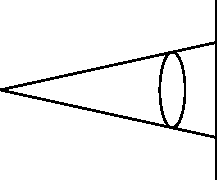
\includegraphics{epee_bocle/bocle_cone_proche}}
	\caption{Cônes de protections pour une bocle tenue loin et près.}
	\label{épée-bocle:fig:bocle-cone}
\end{figure}


\begin{exercice}[Défendre la main]

\D tend le bras droit devant lui et place sa main gauche près de sa main droite. 
\A essaie de toucher la main droite de \D qui ne peut se défendre qu'avec la main gauche.

Cet exercice travaille le fait de placer sa bocle du côté de l'épée adverse et de réagir vite pour l'intercepter.

Source : Arthur.

\end{exercice}


% fluidité
\begin{exercice}[Changements de garde]

Passer d'une garde à une autre en intercalant une frappe à chaque fois.
Chercher à être fluide.

\end{exercice}


\begin{exercice}[Couper la main]

\begin{enumerate}
	\item \A porte une attaque lente à \D, qui se défend simplement.
	\item Si une partie du corps de \A n'est pas protégée, alors \D amène son épée pour le mettre en évidence.
\end{enumerate}

\A peut enchaîner les frappes (en laissant le temps à \D de réagir pour mettre en évidence une éventuelle erreur).
Le but n'est pas d'aller vite mais de vérifier si la position est correcte.

Au début \D peut se concentrer uniquement sur la main d'arme de \A en faisant peu de mouvements, puis quand \A commence à avoir l'habitude \D peut chercher d'autres cibles et bouger légèrement.

\end{exercice}


\subsection{Gardes}


\begin{garde}[Crosse – \emph{Krucke}]
\index{krucke}
\index{garde!épée-bocle!krucke}

Dans la garde de la crosse (all. \emph{Krucke}, ang. \emph{crutch}), les mains sont placées face au visage, la pointe de l'épée vers le bas, la bocle couvrant la main d'arme.

\end{garde}

Cette garde est très hermétique et permet de dévier les estocs bas.


%%%%%%%%%%%%%%
\section{I.33}
%%%%%%%%%%%%%%


% type d'épée : Cinato : XVI, clubs allemands : XIV

% Royal Armouries, Tower Fechtbuch
Le traité MS I.33 (appelé aussi \emph{Walpurgis Fechtbuch} ou \emph{Liber de arte dimicatoria}) est le plus vieux manuel qui nous soit parvenu – il a été rédigé dans la décennie de 1320.
L'auteur serait un prêtre nommé Liutger.

La référence pour l'étude du I.33 est la traduction et le commentaire de Cinato et Suprenant~\cite{cinato:I33:2009}.
Kenner a écrit un manuel sur le sujet~\cite{kenner:I33:2014}.
Les images en couleur peuvent être trouvées sur le site de Wiktenauer~\cite{wiktenauer:I33}.


% TODO: custodia, contraria, liages supérieur/inférieur gauche/droit (inférieur = par en dessous)

\begin{definition}[Assiègement]
\index{assiègement}
\index{obsessio|see{assiègement}}
\index{contraria|see{assiègement}}

Un assiègement (lat. \emph{obsessio}~\cite{cinato:I33:2009}, \emph{contraria}~\cite{kenner:I33:2014}) est une position qui permet de briser une garde (lat. \emph{custodia}).

Il s'agit d'une position relativement hermétique et un assiègement adapté permet de se couvrir des attaques provenant de la garde adoptée par l'opposant.

\end{definition}

% liste des assiègement : krucke


\begin{definition}[Garde – \emph{Custodia}]
\index{garde!I.33}
\index{custodia|see{garde I.33}}

Une garde (lat. \emph{custodia}) est une position permettant de préparer une attaque.
Elle offre généralement une faible protection.

\end{definition}

% liste des gardes : 1 à 7

% TODO: déplacer en épée longue ?
\index{liage}
Il existe quatre liages possible : supérieur/inférieur et gauche/droite.
La personne qui lie est celle qui possède le centre et qui possède donc un avantage (plus ou moins important) sur l'autre.
Lorsque l'épée de celui qui lie est au-dessus on parle de liage supérieur, et de même si l'épée est en-dessous on parle de liage inférieur.
% cf Kenner

\begin{exercice}[Liages]

\begin{enumerate}
	\item \A fait un oberhau.
	\item \D vient prendre un liage.
	\item \A inverse le liage.
\end{enumerate}

L'oberhau est de hauteur variable pour encourager \D à varier les liages.
Le but n'est pas d'aller vite mais de sentir qui a le centre qui lie/est lié, de voir à quel point on est gêné et trouver le meilleur reliage.

\end{exercice}



%%%%%%%%%%%%%%%%%%%%
\section{Liegniczer}
%%%%%%%%%%%%%%%%%%%%


% TODO: add german words in techniques

Le traité de Liegniczer sur l'épée-bocle est très court et contient seulement six enchaînements.
On peut en trouver diverses transcriptions/traductions~\cite{ardamhe:liegniczer, farrell:liegnieczer, lindholm:ringeck_others:2006} ainsi que des interprétations~\cite{farrell:pedagogy_liegnieczer:2014, youtube:sala_armi:liegniczer, youtube:memag:liegniczer, lindholm:ringeck_others:2006, Myers:LiegniczerBuckler, knight:epee_bocle}.
Notre interprétation suit fortement~\cite{youtube:sala_armi:liegniczer, farrell:pedagogy_liegnieczer:2014}, ainsi que~\cite{youtube:memag:liegniczer}.

Le style développé par Liegniczer est très proche du système de Liechtenauer par le fait qu'il repose sur le concept de liage et de winden.
Il se rapproche aussi du I.33 par le fait que la bocle sert avant tout à couvrir la main d'arme, comme cela est indiqué dès le début de la première technique.
Keith Farrell a écrit un article sur la pédagogie de Liegniczer~\cite{farrell:pedagogy_liegnieczer:2014} afin de montrer que la structuration des six techniques présente bien un système cohérent et puissant.

Dans notre interprétation nous nous éloignons du livre de Lindholm, Svard and Clements~\cite{lindholm:ringeck_others:2006} qui ne nous semble pas correspondre tout à fait à l'esprit du système de Liegniczer : par exemple dans la technique 2, l'attaquant et les défenseurs séparent leurs deux mains.
% TODO: citer la page
De même l'interprétation de H.\ Knight~\cite[part I]{knight:epee_bocle} ne nous a pas convaincu, entre autres à cause des positions faibles qu'il adopte.

Dans chaque technique \A attaque tandis que \D est globalement passif : il semble que ce dernier ne soit pas initié à l'escrime et réagisse simplement avec des déflexions.
De même qu'en épée longue, \A va réagir d'une manière différente selon la réaction de \D, en apportant une réponse adaptée au mouvement de \D (ressenti).
% \emph{fühlen}
Ainsi qu'il a été expliqué plus haut, la bocle doit toujours protéger la main d'épée en se plaçant du même côté de l'épée de \D.
De même si \D ne prend pas soin de couvrir son bras alors \A doit frapper cette cible plus facile à atteindre.
Le seul moment où la bocle n'est pas utilisé pour couvrir la main est lorsque \A se trouve près de \D : dans ce cas la bocle est utilisée pour frapper et/ou contrôler les bras/mains de \D (entre autres lorsque l'on change d'axe ou que l'on vient chercher une cible basse).

L'idéal pour pratiquer ces techniques est de décomposer les techniques en séquences où \A doit réagir correctement selon ce que fait \D – d'abord en augmentant progressivement la longueur de l'enchaînement, puis en variant d'une fois à l'autre.


\begin{technique}[Liegniczer 1]
\label{épée-bocle:tech:liegniczer:1}

\A et \D démarrent dans la custodia 2 (épaule droite).

\begin{enumerate}
	\item \A lance un oberhau sur l'épaule droite de \D, en avançant la jambe droite.
	
	\item \D pare avec un oberhau, en avançant la jambe droite, et prend le liage.
	
	\item \alt{Si \D est faible, \A estoque.}
		Si \D est relativement fort au liage, \A exécute un winden en levant les mains en bœuf (en supination ou en pronation).
	
	\item \alt{Si \D ne réagit pas, \A estoque.}
		Si \D pousse la lame vers l'extérieur alors \A quitte le liage et vient frapper \D de l'autre côté en passant sous la lame (\emph{schnappen}),
		tout en frappant les mains de \D avec la bocle pour éloigner la menace.
\end{enumerate}

Au temps 3) le plus simple est de lever directement la main en supination ; cette position est relativement faible si l'on n'utilise pas le pouce en appui comme expliqué dans l'introduction de ce chapitre.
Le \emph{schnappen} au temps 4) sera d'autant plus efficace que \D écarte fort la lame – à l'extrême si \D écarte fort dès le temps 2) alors il n'y a pas de winden.

Pour illustrer nos explications générales, \A n'a pas besoin d'exécuter l'ensemble de la technique si \D fait une erreur.
Par exemple si \D est faible au temps 2) alors \A peut estoquer directement.

Au temps 2) les rôles sont symétriques et \D peut prendre l'initiative, auquel cas les rôles s'inversent.
De ce point de vue une autre manière d'interpréter l'enchaînement est que \D attaque \A qui prend le liage avec un oberhau, et ensuite enchaîne.

\end{technique}


\begin{figure}[htp]
	\centering
	\includegraphics{diagrammes/epee_bocle/liegniczer_1}
	\caption{Diagramme pour la technique 1 de Liegniczer.
	Nous n'indiquons pas le cas où \D ne réagit pas au premier oberhau.}
	\label{épée-bocle:fig:liegniczer:diagramme-1}
\end{figure}



\begin{technique}[Liegniczer 2]
\label{épée-bocle:tech:liegniczer:2}

\A démarre dans la custodia 5 (queue), \D dans la custodia 2 (épaule droite).

\begin{enumerate}
	\item \A lance un unterhau en avançant la jambe droite.
	
	\item \D prend le liage avec un oberhau en avançant la jambe droite.
	
	\item \alt{Si \D est faible, \A estoque.}
		Si \D est fort \A exécute un winden en levant les mains.
	
	\item \alt{Si \D ne réagit pas, \A estoque.}
		Si \D repousse la lame, \A exécute un duplieren tout en se décalant sur la gauche.
		La bocle permet de coincer l'épée de \D.
	
	\item \D se protège du coup et \A vient frapper les jambes du vrai tranchant (dans l'intérieur de \D).
\end{enumerate}

Il est possible d'inverser les temps 1) et 2) si l'on voit l'unterhau de \A comme un liage (inférieur).

\D se trouve naturellement jambe droite devant et il s'agit de la cible principale, alors que le traité indique que \A vise la jambe gauche : une interprétation est que \D peut toujours reculer la jambe droite, mais pas la gauche et si l'on vise cette dernière (ce qui est possible comme le coup est à l'intérieur) alors on est sûr de toucher quelque chose.

\end{technique}

% talhoffer : Myers:LiegniczerBuckler, knight:epee_bocle


\begin{technique}[Liegniczer 3]
\label{épée-bocle:tech:liegniczer:3}
% \index{coup!allemand!wechselhau}

\A et \D démarrent dans la custodia 2 (épaule droite).

\begin{enumerate}
	\item \A lance un oberhau en avançant la jambe droite.
	
	\item Quand \D se protège, \A laisse tomber la pointe de son épée sous celle de \D et la relève ensuite en battant fortement l'épée de \D avec le faux tranchant (coup changeant, wechselhau).
		\A se sert de l'élan pour frapper (du vrai tranchant) la tête de \D du côté droit en avançant la jambe gauche.
	% mouvement de hanches pour le balayage : permet d'éviter l'attaque ?
	
	\item \D se protège et \A exécute un winden en tournant la main en supination.
	
	\item \alt{Si \D ne fait rien, \A estoque.}
		\D dévie l'estoc et \A vient frapper la jambe droite du vrai tranchant.
		La bocle écarte les mains de \D.
\end{enumerate}

Au temps 2) le balayage est exécuté avec le faux tranchant car cela est plus rapide qu'avec le vrai, qui nécessiterait plusieurs rotations du poignet.
Il est aussi important de passer la bocle du côté droit du bras d'arme lors de la frappe, autant pour protéger le bras que pour laisser ouverte la ligne basse d'attaque.

La position en 3) n'est pas très forte : à notre avis l'idée est de surprendre en changeant la ligne d'attaque (technique~\ref{struct:tech:changement-ligne}).

Dans ce contexte la première attaque est une feinte.
Une autre interprétation est possible si \A commence dans la garde du fou : dans ce cas la déflexion en 2) est utilisée contre un oberhau de \D (pour une garde à gauche le balayage se fera naturellement avec le vrai tranchant).

\end{technique}


\begin{technique}[Liegniczer 4]
\label{épée-bocle:tech:liegniczer:4}
% \index{coup!allemand!mittelhau}

\A et \D démarrent dans la custodia 2 (épaule droite).

\begin{enumerate}
	\item \A lance un mittelhau (avec le vrai tranchant) à droite en avançant la jambe droite.
	
	\item \D se protège et \A frappe de l'autre côté avec un second mittelhau (vrai tranchant) en avançant la jambe gauche.
	
	\item \D se protège et \A lance un coup crânien (vrai tranchant) en avançant la jambe droite.
	
	\item \D se protège et \A fait glisser l'épée le long de la bocle de \D pour estoquer le ventre.
		\A garde sa bocle haute pour empêcher \D de baisser ses mains et pour protéger sa tête.
\end{enumerate}

L'idée de l'enchaînement est d'exécuter une série rapide de plusieurs coups qui vise à faire progressivement monter les défenses de \D afin d'attaquer bas à la fin.
Cela marche d'autant mieux si l'on a pu faire entrer \D dans un schéma, par exemple en lançant plusieurs mittelhau à la suite (par exemple avec un enchaînement droit-bas puis gauche-haut).

Les temps 1) et 2) constituent un double zwerchau, où la différence par rapport à l'épée longue est que la première frappe est faite avec le vrai tranchant.
Il est en effet un peu plus difficile de tourner la main sur la garde pour une épée une main puisque la main gauche n'est pas là pour stabiliser, et en gardant le pouce en appui sur les quillons il n'est pas possible de frapper avec le faux tranchant au temps 2) et 3).

Au temps 4) \A ne doit pas ramener son épée en arrière pour estoquer car il perdrait le centre (et du temps).

\end{technique}


\begin{technique}[Liegniczer 4 (variante)]
\label{épée-bocle:tech:liegniczer:4v}

\A et \D démarrent dans la custodia 2 (épaule droite).

\begin{enumerate}
	\item \A lance un mittelhau (avec le faux tranchant) à droite en avançant la jambe droite.
	
	\item \D se protège et \A frappe de l'autre côté avec un second mittelhau (vrai tranchant) en avançant la jambe gauche.
	
	\item \D se protège et \A lance un coup crânien (faux tranchant) en avançant la jambe droite.
	
	\item \D se protège et \A fait glisser l'épée le long de la bocle de \D pour estoquer le ventre.
		\A garde sa bocle haute pour empêcher \D de baisser ses mains et pour protéger sa tête.
\end{enumerate}

La différence avec la variante précédente est que deux des attaques – temps 1) et 3) – se font avec le faux tranchant, et ainsi la première attaque ressemble plus au zwerchau allemand que dans la première version.
Cet enchaînement est possible à condition que le pouce soit placé au niveau de la croix quillons/poignée, comme en épée longue, et que l'on conserve cette position tout le long.

Avec cette tenue la frappe en 3) avec le faux tranchant est très naturelle et plus rapide que si l'on devait ramener le vrai tranchant, et l'on dispose aussi d'un plus grand angle pour estoquer derrière la bocle (du fait de la position du poignet).

% Léo
\end{technique}


Une autre variante est proposée dans~\cite{youtube:sala_armi:liegniczer} : les mittelhaus sont respectivement portés à gauche et à droite.
Nous pensons que cet ordre est moins intéressant car il est quasiment certain qu le coup crânien tombera sur le bouclier ; mais cela reste une variation intéressante qui peut surprendre l'adversaire.


\begin{technique}[Liegniczer 5]
\label{épée-bocle:tech:liegniczer:5}

\A et \D démarrent dans la custodia 2 (épaule droite).

\begin{enumerate}
	\item \A lance un oberhau à droite en avançant la jambe droite, et tout en frappant tourne son poignet de 90° (sens direct) pour amener la pointe vers le bas, derrière le bouclier de \D (coup plongeant, sturtzhau).
	
	\item \alt{Si \D ne fait rien, \A estoque.}
		\D dévie l'estoc et \A fait contourne la bocle avec sa pointe pour venir estoquer le ventre : soit en descendant (rotation du poignet), soit en montant (rotation de l'épaule).
	
	\item \alt{Si \D ne fait rien, \A estoque.}
		\D dévie l'estoc (par exemple en passant en \emph{Krucke}) et \A exécute un winden en tournant la main en supination.
	
	\item \alt{Si \D ne fait rien, \A estoque.}
		\D dévie l'estoc vers sa droite et \A vient frapper la jambe droite du vrai tranchant.
		La bocle écarte les mains de \D.
\end{enumerate}

Au temps 1) l'oberhau est une feinte (mais si \D ne bouge pas alors il n'y a pas besoin de l'exécuter).
La fin de la technique est très similaire à celle de la séquence~3 (technique~\ref{épée-bocle:tech:liegniczer:3}).

Comme indiqué en 2) le contournement de la bocle peut se faire de deux manières.
Plusieurs interprétations favorisent un estoc descendant (en rapport avec la variante suivante), mais l'estoc montant semble favorisé dans la traduction de l'\textsc{Ardamhe}~\cite{ardamhe:liegniczer} : "monte la pointe par dessous".

Au temps 3) nous avons noté qu'une bonne défense pour \D est le \emph{Krucke}.
Elle est particulièrement adaptée si l'estoc est bas, mais elle ne correspond pas à une défense "naïve".
En Krucke \D peut sembler être protégé aux jambes : en fait lorsqu'il dévie l'estoc il commence à s'ouvrir, et la bocle permet d'écarter encore plus sa lame.

\end{technique}


\begin{technique}[Liegniczer 5 (variante)]
\label{épée-bocle:tech:liegniczer:5v}

\A et \D démarrent dans la custodia 2 (épaule droite).

\begin{enumerate}
	\item \A lance un oberhau à droite en avançant la jambe droite, et tout en frappant tourne son poignet de 90° (sens direct) pour amener la pointe vers le bas, derrière le bouclier de \D (coup plongeant, sturtzhau).
	
	\item Avant que \D ne dévie la pointe, \A contourne la bocle de \D grâce à une rotation du poignet, afin d'estoquer le côté droit de \D.
	
	\item \alt{Si \D ne fait rien, \A estoque.}
		\D dévie l'estoc et \A exécute un winden en tournant la main en supination.
	
	\item \alt{Si \D ne fait rien, \A estoque.}
		\D dévie l'estoc vers sa droite et \A vient frapper la jambe droite du vrai tranchant.
		La bocle écarte les mains de \D.
\end{enumerate}

Dans cette variante \A exécute deux feintes : d'abord en inversant la direction de la lame, puis en contournant la bocle.
Dans ce cas-là l'estoc au temps 2) est plus haut et \D devra utiliser une garde haute pour le dévier.

\end{technique}

\begin{figure}[htp]
	\centering
	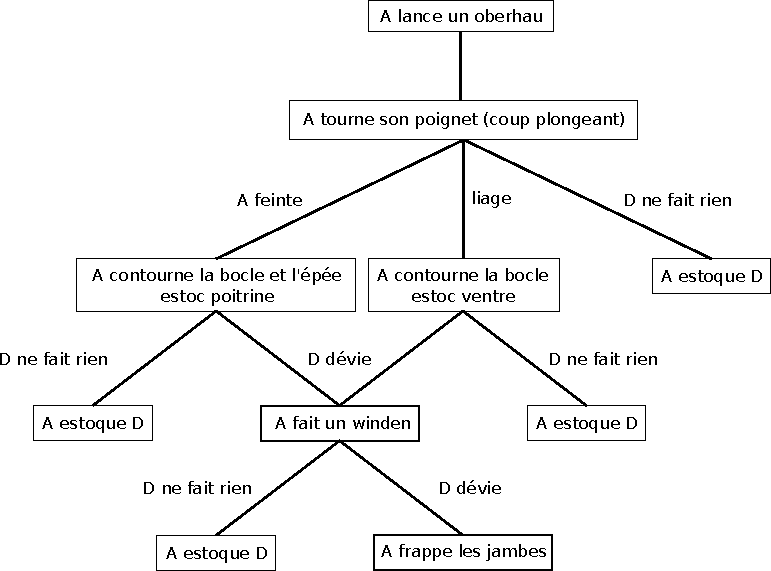
\includegraphics{diagrammes/epee_bocle/liegniczer_5}
	\caption{Diagramme pour la technique 5 de Liegniczer.}
	\label{épée-bocle:fig:liegniczer:diagramme-5}
\end{figure}


\begin{technique}[Liegniczer 6]

\A démarre dans une garde basse, \D dans la custodia 2 (épaule droite).

\begin{enumerate}
	\item \D lance un oberhau à droite en avançant la jambe droite.
	
	\item \A passe en demi-épée et fait une parade franche.
	
	\item \A lâche sa main droite et attrape la bocle de \D.
	
	\item \A arrache la bocle de \D.
	
	\item \A utilise la bocle pour frapper \D au visage.
\end{enumerate}

La meilleure manière pour retirer la bocle est de l'attraper par en-dessous (avec la paume tournée vers la droite) et de tourner dans le sens horaire~\footnotemark{}.
\footnotetext{Attention en pratiquant avec un partenaire : s'il a des gants épais ils peuvent rester coincés sous la poignée et la torsion peut être douloureuse.}

\A peut directement démarrer en demi-épée mais son intention peut alors être devinée plus facilement, sauf si la main est cachée par la bocle – par exemple grâce à la custodia 1 (sous le bras) ou si l'échange commence hors distance et \A adopte une position reposante.

À partir du moment où \A lâche sa poignée il doit la garder hors d'atteinte de \D.

\end{technique}


\chapter{Pertuisane}

\section{Saviolo}

Dans ce style de combat l'idée est de se déplacer sur un cercle. Au début d'une série, le pied ne se pose pas complètement (i.e. seul le talon est posé) afin de permettre de changer facilement de direction ou de cible.

La main gauche est très mobile (donc pas nécessairement verrouillée à la hanche ou à la tête) et permet de changer la position de la pointe. Ainsi avec la main au niveau de la hanche la tête de l'arme est vers le haut, et inversement avec la main près de l'épaule la pointe est vers le bas.

Au moment où l'un des deux adversaires a sa hampe en contact avec celle de l'autre il peut en profiter pour faire levier et l'écarter ou la coincer au sol. Dans ce dernier cas il ne reste plus qu'à ramener l'arme pour trancher au visage.

\begin{exercice}
\begin{enumerate}
	\item \A et \D se font face, pieds droits en avant, l'arme à l'intérieur de l'autre.
	
	\item \A fait un pas sur la droite (le pied gauche est immobile) ; seul le talon est posé. En remontant la main gauche, il fait passer la pointe sous l'arme de \D et vient battre celle-ci pour l'écarter.
	
	\item \A avance encore son pied et estoque au niveau du ventre (main gauche au niveau de la tête).
	
	\item \D lève sa main gauche et ramène sa pertuisane pour se protéger du coup.
	
	\item \alt{Si \A ne réagit pas, \D écarte l'arme \A et l'amène au sol avant de le trancher avec son arme.}
\end{enumerate}

Noter que le pied arrière de \A ne bouge à aucun moment.

Source : Paul et Raphaël (ENS), d'après~\cite{livermore:cornucopia:partizan:2014}.
\end{exercice}

\begin{exercice}
Cet exercice commence comme le précédent, mais l'attaque de \A au point 3) est une feinte.
\begin{enumerate}
	\item \A et \D se font face, pieds droits en avant, l'arme à l'intérieur de l'autre.
	
	\item \A fait un pas sur la droite, passe sa pertuisane sous celle de \D et l'écarte d'un batté.
	
	\item \A fait comme s'il allait porter un estoc (descendant) mais n'avance pas le pied.
	
	\item \D lève la main gauche pour parer l'estoc avec la hampe.
	
	\item Avant le contact avec la hampe de \D, \A ramène sa main gauche au niveau de la hanche pour faire passer son arme au-dessus de celle de \D afin de l'abattre sur le bras de \D.
	
	\item \D se protège en tournant les hanches vers la droite.
\end{enumerate}

Le déplacement du pied à l'avant-dernier temps (5) n'est pas clair. On peut déplacer le pied gauche sur le côté. On peut aussi ne pas bouger, ou bien avancer le pied droit (ce dernier mouvement peut être dangereux car la tête de la pertuisane de \D peut être très proche). Finalement Raphaël faisait un pas sur le côté en croisant les bras (à l'allemande).

Pour réussir à se protéger au temps (6), il faut pour cela que \D ne se soit pas précipité sur son premier contre et qu'il ait bien avancé le pied droit afin de gagner le temps nécessaire.

Source : Paul et Raphaël (ENS), d'après~\cite{livermore:cornucopia:partizan:2014}.
\end{exercice}

\chapter{Lance}


\section{Généralités}

% Romain
La lance est une arme qui doit être très mobile et offensive.
Pour cette raison il n'est souvent pas intéressant de verrouiller la main (contre la hanche ou a tête) afin de pouvoir changer rapidement de direction d'attaque.
De plus en bougeant souvent la lance l'adversaire aura peu l'occasion de la dégager via un enroulé ; de même il sera beaucoup plus simple de ramener la pointe dans le centre si l'adversaire porte un coup puissant contre le manche.
Au contraire le verrouillage pourra être utile dans les formations serrées (par exemple de piquiers~\footnotemark).
\footnotetext{Ceux-ci verrouillaient le manche en le posant sur leur ceinture, qui était portée plus haut que nous.}
% ~\footnote{Une poussée par des lanciers peut désorganiser un mur de boucliers.}

La lance peut aussi être tenue de deux manières, comme le bâton long : toutefois on observera le plus souvent la tenue où les deux pouces sont tournés du même côté.
Cette tenue facilite aussi le fait de coulisser la lance dans la main avant afin de porter un estoc tout en gagnant de l'allonge.

% TODO: gardes

\begin{coup}[Attaque basse]
En garde basse, la main avant est la même que celle du pied avant.
Avancer le pied avant et faire coulisser le manche dans la main avant pour estoquer.
\end{coup}


\begin{coup}[Attaque haute]
En garde haute, la main avant est la même que celle du pied avant.
Avancer le pied avant et faire coulisser le manche dans la main avant pour estoquer.
La lance a une direction descendante.
\end{coup}

Cette seconde attaque est utile pour piquer derrière un bouclier, à la tête.

\begin{technique}[Retour en garde haute]
Après une attaque basse, monter la main arrière et descendre sur les appuis.
La main avant se place sous la hampe pour protéger les doigts (si prise bâton, placer le poing).

Une amélioration consiste à placer l'avant bras.
\end{technique}

Dans la garde précédente où l'avant-bras est placé contre le manche, avec une hallebarde on est alors très bien placé pour frapper avec le tranchant par en haut.

\begin{technique}[Retour en garde basse]
Après une attaque haute, faire un tour avec la pointe en tournant la main gauche (arrière) dans le sens antihoraire (comme un rameur), et revenir en garde basse en ramenant la main en bas.
Le tour permet de reprendre le centre, sinon la lance peut se retrouver à l'extérieur.
Et si l'autre n'est pas prudent il est possible de le planter direct.
\end{technique}


\section{Lance contre épée courte}


\begin{exercice}

\A porte l'épée.

\begin{enumerate}
	\item \A part en garde de quarte (pied droit en avant) ou de tierce (gauche en avant) et change de garde en faisant passer son épée sous la lance.
\end{enumerate}

Le centre de gravité de l'épée reste fixe, et la lame doit rester tout le temps en contact avec la hampe de la lance pour garder le contrôle.

Le lancier peut aussi avancer pour compliquer l'exercice.
\end{exercice}


\begin{technique}

\D est armé de la lance et démarre pied gauche devant.
\A démarre pied droit devant.

\begin{enumerate}
	\item \A vient bloquer en tierce la lame.
	
	\item \A passe rapidement sous son bras droit en passant le pied gauche devant, pour ensuite frapper \D.
\end{enumerate}

Le temps 1) est une feinte qui laisse croire au lancier qu'il va pouvoir l'embrocher.
\end{technique}


\begin{technique}

\D est armé de la lance.

\begin{enumerate}
	\item \D recule en donnant des coups d'estoc.
	
	\item \A fait semblant de frapper au poignet par la droite, en tenant son épée de manière à écarter la pointe.
	
	\item En passant la lame par en dessous, \A dégage la lance en octave et attaque le lancier.
\end{enumerate}
\end{technique}


\section{Lance contre épée longue}

% Romain
Les épées longues utilisées dans ce genre de combat (au moins au début) étaient d'une taille similaire à celles des épées longues italiennes.
Ce n'est que plus tard qu'elles évolueront vers les épées à deux mains (comme par exemple l'espadon).

\index{ricasso}
Ces lames comportent un ricasso, c'est-à-dire une partie émoussée (et éventuellement recouverte de cuir) située au-delà des quillons.
Cette partie se termine par des ergots qui permettent de délimiter les différentes zones, de servir de point de repère (quand on plaque la lance au sol, on peut savoir plus facilement à quelle hauteur elle se trouve) et d'accrocher les manches.
Le ricasso permettait de raccourcir la prise sur la lame tout en offrant une meilleure sécurité : en effet dans le type de combat dont il est question, il pouvait arriver que l'on se retrouve en contact avec son épée – par exemple en parant en prime avec le haut de la lame contre l'épaule.


\begin{technique}

\A est armé de la lance.

\begin{enumerate}
	\item \A porte un coup de lance bas.
	
	\item \D sort sur son pied gauche et pare en sixte.
	
	\item \D avance le pied droit et appuie sur le manche de la lance avec son épée, direction à 90° pour l'enfoncer dans le sol.
	Les mains sont loin devant pour gêner \A.
	
	\item \D avance le pied gauche et avance son tranchant contre D.
\end{enumerate}

Parer avec le faux tranchant permet d'avoir une rotation plus naturelle au temps suivant. 
À la fin \D doit être prêt à suivre \A s'il recule.

Source : Romain.
\end{technique}


\begin{technique}

\A est armé de la lance.

\begin{enumerate}
	\item \A porte un coup de lance haut.
	
	\item \D engage son épée en bœuf~\footnotemark, pied gauche en avant.
	\footnotetext{À voir plus comme un estoc dans le vide que comme une quinte.}
	
	\item \D avance son bras gauche sous son épée pour attraper le manche.
	
	\item \D donne un coup dans les tibias de \A.
\end{enumerate}

L'inertie permet d'avoir un coup efficace même avec une main (en demi-armure typique de l'époque les tibias ne sont pas protégés).
Il faut être haut pour ne pas permettre à l'autre d'avoir la tête.

Source : Romain.
\end{technique}


\begin{technique}

\A est armé de la lance.

\begin{enumerate}
	\item \A porte un coup de lance haut.
	
	\item \D engage son épée en bœuf, pied gauche en avant.
	
	\item Avancer le pied droit et frapper parallèlement au manche. 
\end{enumerate}

Ce coup permet d'avoir au moins les mains, sinon la tête, et de gêner \A.
Il peut se faire sur une mauvaise parade, par exemple où l'épée est contre l'épaule.

Source : Romain.
\end{technique}


\begin{technique}

\A est armé de l'épée longue.

\begin{enumerate}
	\item \A prend le contact avec la lance en quarte.
	
	\item \A passe par dessus la lance en octave.
	
	\item \A avance le pied droit.
	
	\item \A avancer le pied gauche et frappe.
\end{enumerate}

Cette technique est très surprenante car le coup arrive du côté opposé à celui prévu.

Il est possible de passer en quarte après avoir paré un coup d'estoc en tierce, par exemple.

Source : Romain.
\end{technique}


\subsection{Bataille rangée}


\begin{technique}[Pénétrer un mur de lanciers]

\A fait face à trois lanciers, \Dn2 en face de lui, \Dn1 à la droite de celui-ci et \Dn3 à sa gauche.

\A ne doit pas chercher à attaquer directement \Dn2 car ce dernier pourra se protéger facilement, et \A recevra un coup de \Dn1 et \Dn3.
Au lieu de cela il doit chercher à dégager la lance de \Dn1 – si possible en écartant aussi celle de \Dn2, voire d'autres lanciers – pour ensuite frapper à droite en visant les mains de \Dn3 pour l'empêcher de le frapper.

Quand les lances sont écartées alors les alliés de \A (par exemple des lanciers) peuvent entrer dans le combat.

Le temps dont il dispose pour bloquer le coup de \Dn3 est très court.

Source : Romain.
\end{technique}



\section{Lance contre épée-bouclier}


Certaines techniques d'épée longue peuvent aussi s'utiliser.

% Romain
Contre un fantassin armé d'un bouclier, un lancier a trois cibles :
\begin{enumerate}
	\item la tête, par dessus le bouclier ;
	\item les jambes du côté du bouclier (zone définie par là où le bouclier ne peut pas voir) ;
	\item le ventre, entre l'épée et le bouclier.
\end{enumerate}
% attaque vers l'avant en faisant coulisser ;
% en se déplaçant sur la gauche et en s'accroupissant, contourner le bouclier par le bas et attaquer en remontant (par exemple en passant sous la cotte de mailles) ;
% en se déplaçant sur la droite, contourner le bouclier par le haut et attaquer bras tendus.


\begin{garde}
Contre une attaque de lance à la tête, \D tient le bouclier en avant (mais pas complètement, sinon D peut passer en dessous), et place son épée au dessus.

Source : Romain.
\end{garde}


% Romain
L'épéiste ne doit jamais se trouver face à la pointe de la lance, comme le lancier peut rapidement piquer.
Si une épée fait face à une lance, c'est en général une bonne idée de glisser le long du manche pour avoir les doigts du lancier.

Quand le lancier attaque le but du défenseur est de coincer le manche de la lance sous l'umbo afin de la contrôler et de la baisser (pour la planter dans le sol, marcher dessus…).
Si le lancier voit que sa lance se plante dans le sol, alors il doit la basculer comme un levier (en se servant du côté planté dans le sol) pour venir plaquer le bouclier adverse contre son corps
Là il peut dégainer son sax (porté à la ceinture ou tenu en même temps que la lance dans la main droite) pour poignarder.
Il peut être nécessaire d'inverser le sens de la prise de la main droite pour obtenir un meilleur levier.
Le lancier a intérêt de rester très loin ou très près de son adversaire, tandis que la moyenne distance convient à l'épéiste.


\begin{technique}
Quand \D pare un coup de lance au niveau du ventre, il doit appuyer avec son bouclier sur le manche pour enfoncer la lance dans le sol.

Source : Romain.
\end{technique}


\begin{exercice}
\A a la lance.

\begin{enumerate}
	\item \A fait un estoc haut en visant le visage.
	
	\item \D se protège.
	
	\item \A revient en garde et estoque \D au ventre, à l'ouverture apparue après qu'il ait levé le bouclier.
	% avec la technique ...
	
	\item \D se protège.
\end{enumerate}

Source : Romain.
\end{exercice}


\begin{technique}
\A est armé de l'épée et du bouclier.

\begin{enumerate}
	\item \A vient prendre le contact avec la lance par en dessous, sans trop avancer.
	
	\item \A avance loin le bouclier pour dévier la lance sur le côté gauche, tout en faisant un pas.
	La partie latérale du bouclier est en contact, pas le haut.
	Avancer le pied.

	\item \A frappe \D au tibia.
\end{enumerate}

Le premier mouvement est comme un un estoc dans le vide.

Source : Romain.
\end{technique}


\section{Lance contre autre arme}


\begin{technique}
\D est armé d'un sabre d'abordage.

\begin{enumerate}
	\item \A fait une attaque haute.
	
	\item \D Pare en quinte, pointe vers l'avant (main du côté droit).
	
	\item \D fait un tour complet autour de sa jambe droite en ramenant le sabre contre son côté, pointe derrière son dos.
	
	\item \D estoque \A au ventre.
\end{enumerate}

Il s'agit d'une des rares techniques avec un tour sur soi-même.

Source : Romain.
\end{technique}


\section{Lance-bouclier contre épée longue}


\begin{technique}

\A est armé de l'épée longue.

\begin{enumerate}
	\item \A prend le contact avec la lance en tierce menaçante.
	
	\item \A décale l'épée sur la droite en passant derrière le bouclier, et frappe sur le côté gauche du cou.
	Les quillons sont horizontaux pour bloquer le bouclier.
	
	\item \alt{Si \D garde sa lance et son bouclier serré, passer en bœuf pour frapper à la tête.
	Le bouclier est bloqué par l'épée.}
	
	\item Dans tous les cas, si \D lève le bouclier pour se protéger la tête, se décaler sur la droite et frapper les jambes.
\end{enumerate}

Si \A ne bloque pas le bouclier il risque de se prendre un coup.

Source : Romain.
\end{technique}



\begin{technique}

\A est armé de l'épée longue.

\begin{enumerate}
	\item \A essaie de prendre le contact avec la lance en tierce mais échoue en passant trop court.
	
	\item \A exécute un coup tordu sur la droite pour plaquer la lance sur le sol.
	
	\item \A frappe \D à la tête avec un estramaçon en avançant vers lui.
\end{enumerate}

Au dernier coup \A doit être près de \D et être prêt à lui tourner autour pour éviter de se prendre un coup.

Source : Romain.
\end{technique}

\chapter{Rapière}


%%%%%%%%%%%%%%%%%%%%%
\section{Généralités}
%%%%%%%%%%%%%%%%%%%%%


\begin{technique}

\A se laisse tomber au sol tout en mettant un estoc en mettant sa jambe gauche loin en arrière et en s'appuyant par terre avec sa main gauche.

La main droite doit se trouver au-dessus de la tête pour la protéger.

% Source : Romain.
\end{technique}


%%%%%%%%%%%%%%%%%%
\section{Destreza}
%%%%%%%%%%%%%%%%%%


Le concept principal est celui de premier plan : il s'agit du plan qui joint les deux adversaires.
Le pied avant est toujours pointé vers l'adversaire.
Il y a parfois des postures bizarres (avec peu d'équilibre...) mais elles ne sont pas faites pour y rester.

Trois dégagements sont possibles pour reprendre le centre :
\begin{enumerate}
	\it
	\item faire passer la lame sous celle de l'autre, avec un mouvement du poignet ;
	\item demi-taille : ramener l'épée en arrière et la faire passer par dessus l'autre dès que possible, encore avec le poignet ;
	\item comme précédent mais avec un tour complet par le bas, et là le bras est plus impliqué.
	% couronné ?
\end{enumerate}


\begin{garde}

L'épée est horizontale, à hauteur de visage, les quillons perpendiculaires au sol.
La coque protège bien le visage.
\end{garde}


\begin{garde}

Le bras est un peu plié, la lame se trouve dans le prolongement de l'avant-garde.
\end{garde}

Cette seconde garde permet de placer le fort contre le faible.


\begin{technique}
\A et \D sont en garde 1.

\begin{enumerate}
	\item \A passe en garde 2 afin de prendre le faible.
	\item \A passe le pied avant sur le côté où se trouve la lame de \D, et le tourne vers \D.
	\item \A ramène le pied arrière.
	\item \A fente pour estoquer \D.
	\item \D fait un dégagement en se déplaçant dans le même sens que \A.
	\item \D estoque.
\end{enumerate}

% Source : Jan.
\end{technique}


%%%%%%%%%%%%%%%%%%%%
\section{Capo Ferro}
%%%%%%%%%%%%%%%%%%%%


Le contrôle de la lame adverse est obtenu en étant très près de lui.
Ainsi tout attaque de termine en avançant vraiment sur l'autre.
Lever la main et estoquer vers le bas permet d'être bien couvert.

Pour dérouter l'adversaire on peut passer d'une ligne d'attaque haute à une ligne basse.
Par exemple en boxe : si \A donne des coups de poings sans s'arrêter, \D ne peut pas espérer contrer en frappant des poings.
Mais il peut donner un coup de pied là où l'attention de \A n'est pas, et après il peut frapper du poing.


\begin{technique}

\begin{enumerate}
	\item \A avance et estoque.
	\item \D passe sous la lame de \D si elle est à gauche, et vient battre en quarte, tout en faisant un quarter du pied.
	\item \D estoque le côté droit de \A en ayant la main haute.
\end{enumerate}

En combat libre, le coup du berger pour \A est d'attendre loin avant d'avancer en accélérant pour estoquer : la technique actuelle est un bon contre.

% Source : Romain.
\end{technique}


\begin{technique}

\begin{enumerate}
	\item \A attaque \D à la tête avec un coup tranchant.
	\item \D se protège en quinte.
	\item \D fait passe sa pointe par dessus le bras de \A et laisse tomber sa pointe en appuyant sur la lame.
	\item \D monte sa pointe en baissant sa main et estoque \A à l'aisselle droite.
	\item Pour se protéger, \A peut exécuter la technique précédente.
\end{enumerate}

Au temps 3) la pointe de \D doit se trouver légèrement derrière la main de \A pour éviter les quillons, et avoir le fort bien placé. Mais il ne faut pas être trop loin non plus.

Au temps 4) \D doit garder un contact avec la lame de \A pour la contrôler, sinon il pourra caver. Il ne faut pas non plus appuyer trop sinon À aura de l'élan pour donner un coup de taille.

Une autre défense plus risquée est de décaler en quadrant en se protégeant en prime.
La parade franche en 2) semble du pain béni pour A, car il est très facile de reprendre le dessus.

% Source : Romain.
\end{technique}


\begin{technique}

\begin{enumerate}
	\item \A est en garde type destreza et empêche \D d'avancer (plus grande allongé, etc.).
	\item \D fait une feinte en avançant comme pour un estoc.
	\item \D prend le contact en quarte (ou se protège si \A a réagi).
	\item \D décale à gauche et passe en seconde.
	\item \D baisse la main et estoque en montant.
\end{enumerate}

% Source : Romain.
\end{technique}


%%%%%%%%%%%%%%%%%%%%%%%%%%%
\section{Thibault d'Anvers}
%%%%%%%%%%%%%%%%%%%%%%%%%%%


Il faut prendre une posture détendue.
Les déplacements se font en marchant normalement, la lame est tenue tranquillement~\cite{guidoux:dijon:thibault:2015}.
L'arme se tient légèrement tournée par rapport à la prise classique, le plat de la lame est parallèle au sol, l'arceau se trouve à droite. Le pouce se trouve sur le plat de la lame au delà des quillons et forme un crochet avec l'index.
À la rapière la distance est bonne si le bout de la lame touche la coquille de l'autre quand les armes sont tenues parallèles au sol.


\begin{technique}

En garde pied droit devant, lames au contact.

\begin{enumerate}
	\item \A tend la rapière devant lui.
	\item \A estoque, tandis que \D écarte très légèrement la lame de \A et fait un léger pas sur la gauche (environ \SI{5}{cm}) tout en tendant le bras pour estoquer au visage.
\end{enumerate}

% \source{\cite{guidoux:dijon:thibault:2015}}
\end{technique}


\begin{technique}

En garde pied droit devant, lames au contact.
\D possède une rapière et une dague.

\begin{enumerate}
	\item \A tourne légèrement le poignet (pouce vers la gauche) et tourne dans le sens horaire autour de \D.
	\item Quand il se trouve à 90°, \A estoque \D au niveau de l'aisselle (ou de la poitrine droite).
\end{enumerate}

Il est très difficile de parer un coup à cet endroit avec la dague.
\A doit exercer une très légère pression, sinon \D aura envie de caver.

% \source{\cite{guidoux:dijon:thibault:2015}}
\end{technique}


\begin{technique}

\A est en garde pied droit devant, \D est pied gauche devant, les lames sont en contact.
\D possède une rapière et une dague, et les tient avec la pointe au même niveau.

\begin{enumerate}
	\item \A tourne légèrement le poignet (pouce vers la gauche) et tourne dans le sens horaire autour de \D.
	\item \D donne un coup de dague vers la droite pour chasser l'épée de \A.
	\item \A laisse sa lame partir en un cercle autour de sa tête, tout en tournant autour de \D par la droite (inversion du sens).
	\item Quand sa lame se trouve à sa droite, \A resserre les doigts et effectue un estoc montant.
\end{enumerate}

Pour un cercle efficace \A doit détendre ses doigts.

% \source{\cite{guidoux:dijon:thibault:2015}}
\end{technique}


\begin{technique}

En garde pied droit devant, lames au contact.
\D possède une rapière et une dague.

\begin{enumerate}
	\item \A tourne légèrement le poignet (pouce vers la gauche) et tourne dans le sens horaire autour de \D.
	\item \D écarte légèrement la lame de \A vers la gauche avec sa dague.
	\item \A avance légèrement et tend le bras pour menacer \D et le faire accentuer son geste d'écart.
	\item \A tourne autour de \D par la droite, en quartant du pied et lève la main pour faire un estoque descendant.
	\item \A ramène sa main vers le bas et pousse vers la gauche afin d'estoquer \D par en-dessous.
\end{enumerate}

% \source{\cite{guidoux:dijon:thibault:2015}}
\end{technique}


%%%%%%%%%%%%%%%%
\section{Divers}
%%%%%%%%%%%%%%%%


Les quatre techniques suivantes sont inspirées du messer~\cite{kleinau:dijon:rapier_messer:2015}.
Il s'agit de la variation d'une même technique où la conclusion dépend de :
\begin{itemize}
	\item de la distance entre \A et \D ;
	\item si \A possède ou non une dague.
\end{itemize}


\begin{technique}

\A n'a pas de dague et reste loin au temps 2).
\D est en prime.

\begin{enumerate}
	\item \A lance un oberhau et \D pare en quinte de pied ferme, tout en gardant la main gauche à proximité.
	
	\item \D vient saisir le poignet de \A.
	
	\item \D tire par le poignet et percute le coude avec le pommeau (côté ou extérieur).
	
	\item \D pousse \A (qui a le bras tendu et donc suit juste), et ensuite D franche.
\end{enumerate}

Au temps 3) pour bloquer l'articulation, \D peut aussi venir serrer avec le pommeau contre son avant-bras.

% Source : \source{Jan, d'après~\cite{kleinau:dijon:rapier_messer:2015}}
\end{technique}


\begin{technique}

\A n'a pas de dague et se trouve près au temps 2).
\D est en prime.

\begin{enumerate}
	\item \A lance un oberhau et \D pare en quinte de pied ferme, tout en gardant la main gauche à proximité.
	
	\item \D vient saisir le poignet de \A.
	
	\item \D remonte la main de l'autre au dessus de la tête voire derrière, puis recule bien la main pour estoquer visage.
\end{enumerate}

% Source : \source{Jan, d'après~\cite{kleinau:dijon:rapier_messer:2015}}
\end{technique}


\begin{technique}

\A a une dague et reste loin au temps 2).
\D est en prime.

\begin{enumerate}
	\item \A lance un oberhau et \D pare en quinte de pied ferme, tout en gardant la main gauche à proximité.
	
	\item \D vient saisir le poignet de \A.
	
	\item \D repousse \A, puis part vers la gauche et estoque sous le bras droit.
\end{enumerate}

% Source : \source{Jan, d'après~\cite{kleinau:dijon:rapier_messer:2015}}
\end{technique}


\begin{technique}

\A a une dague et se trouve près au temps 2).
\D est en prime.

\begin{enumerate}
	\item \A lance un oberhau et \D pare en quinte de pied ferme, tout en gardant la main gauche à proximité.
	
	\item \D vient saisir le poignet de \A.
	
	\item \D lève la main de \A puis se déplace sur la gauche pour trancher derrière le genou droit.
\end{enumerate}

% Source : \source{Jan, d'après~\cite{kleinau:dijon:rapier_messer:2015}}
\end{technique}


\chapter{Messer}


Le faux tranchant d'un messer est tranchant sur la toute dernière partie (\SI{10}{cm}). La prise se fait comme le sabre.
Après une attaque on casse le poignet pour étendre l'arme et trancher.
Globalement la main gauche reste en arrière.


%%%%%%%%%%%%%%%%%%%
\section{Leküchner}
%%%%%%%%%%%%%%%%%%%
\label{sec:messer:lekuchner}


Les techniques qui suivent sont similaires aux exercices~\ref{mains-nues:ex:enzi-1}, \ref{mains-nues:ex:enzi-2}, \ref{mains-nues:ex:enzi-3} et \ref{mains-nues:ex:enzi-4}.


\begin{technique}

\D démarre en garde du fou.

\begin{enumerate}
	\item \A attaque à la tête.
	\item \D recule et lève son messer pour couper sous le bras de \A avec le faux tranchant.
	\item \D revient en garde haute en reculant.
	\item \D recule encore en laissant bien son messer.
\end{enumerate}

Le but final est d'avoir un grand angle avec la direction de l'attaque afin de heurter le bras plus efficacement (sinon risque d'être parallèle à la lame).
En principe le coup est très fort, et on peut tester en visant le messer de l'autre plutôt que le bras. Pour que le pouce n'ait pas mal on abandonne la prise sabre, en le faisant glisser sur le côté.
Si \D ne revient pas en garde et qu'il a raté alors \A a la possibilité de revenir en estoc.
Fonctionne quelque soit le pied de départ et le côté où l'on part.

Source :~\cite{enzi:dijon:messer_inner:2015}.

\end{technique}


\begin{technique}

\D démarre en garde du fou.

\begin{enumerate}
	\item \A attaque à la tête.
	\item \D esquive sur le côté et coupe le poignet de \A avec le vrai tranchant.
	\item \D revient en garde haute et recule.
\end{enumerate}

La main se trouve du côté où l'on sort.

Source :~\cite{enzi:dijon:messer_inner:2015}.

\end{technique}


\begin{technique}

\D démarre en garde du fou.

\begin{enumerate}
	\item \A attaque à la tête.
	\item \D esquive sur le côté et frappe le poignet de \A avec le vrai tranchant.
	\item \D avance et appuie sur le poignet en coupant.
\end{enumerate}

Source :~\cite{enzi:dijon:messer_inner:2015}.

\end{technique}


\begin{technique}

\D démarre en garde du fou.

\begin{enumerate}
	\item \A attaque à la tête.
	\item \D pare en bœuf à gauche, en se déplaçant légèrement à gauche.
	\item De la main gauche \D pousse la main de \A un peu vers la droite.
	\item \D défend des doigts et envoie son pommeau dans la tête de \A.
	\item \D se sert du choc pour faire tourner son messer en reculant et frappe \A au visage du tranchant.
\end{enumerate}

En fait au temps 2) ce n'est pas un vrai bœuf : il s'agit juste de lever l'arme droit pour accrocher l'arme de \A dans le troisième clou.
Avant 3) \D regardait \A à droite de son bras, après 3) il le regarde à gauche.

Source :~\cite{enzi:dijon:messer_inner:2015}.

\end{technique}


\begin{technique}

\D démarre en garde du fou.

\begin{enumerate}
	\item \A attaque à la tête.
	\item \D se protège en quinte en avançant, pied gauche devant.
	\item \D heurte la main droite de \A avec sa main gauche pour écarter sa lame, tandis que de la main droite il tranche au visage.
\end{enumerate}

Le mouvement en 2) est l'éternel écartement des épaules cher à Romain.
En 3) Enzi conseille de reculer.

Le mouvement du corps est le même que l'exercice~\ref{mains-nues:ex:enzi-2}.

Source :~\cite{enzi:dijon:messer_inner:2015}.

\end{technique}


\begin{technique}

\D démarre en garde du fou.

\begin{enumerate}
	\item \A attaque à la tête.
	\item \D se protège en quinte en avançant, pied gauche devant.
	\item Du tranchant de la main \D percute l'avant bras de \A.
	\item \D ramène son bras gauche, en accrochant éventuellement le pommeau de \A, et pousse avec le bras droit pour écraser le messer de \A et trancher au visage de \A.
\end{enumerate}

Il est important de ne pas chercher à saisir le pommeau : le placement est tel que le messer adversaire sera soit hors portée, soit retenu par la main. Le coup se fait entre le poignet et le coude.
Au dernier temps \A va en général se faire trancher aussi par le faux tranchant de sa propre arme.
% TODO: Le mouvement d'écartement est toujours celui de Romain.

Source :~\cite{enzi:dijon:messer_inner:2015}.

\end{technique}


\begin{technique}

\D n'a pas d'arme.

\begin{enumerate}
	\item \A attaque à la tête.
	\item \D part sur la gauche et couvre avec son bras droit, main vers le haut.
	\item \D éjecte le bras de \A avec un mouvement circulaire dans le sens horaire.
	\item \D frappe \A.
\end{enumerate}

L'objectif au temps 2) est de parvenir à arriver avec l'avant-bras contre le plat de la lame.
Voir l'exercice~\ref{mains-nues:ex:enzi-4}.

Source :~\cite{enzi:dijon:messer_inner:2015}.

\end{technique}



% épée longue en armure ?


\part{Étude : arts modernes}

\chapter{Close combat}

Fairbairn constitue une référence sur le close combat~\cite{fairbairn:allin:2008}.

% TODO: défense sur la saisie

% à terre : technique du ciseau

\section{Étranglements}

Pour limiter l'efficacité d'un étranglement, il faut monter les épaules et rentrer le menton.
Ceci est sous-entendu sur toute défense d'étranglement.


\begin{technique}[Étranglement arrière]

\begin{enumerate}
	\item \A arrive derrière \D pour l'étrangler avec le bras droit.
	
	\item Dès qu'il sent le début de l'étranglement, \D vient placer sa main droite dans le creux du coude de \A, à l'intérieur.
	
	\item \D attrape de sa main gauche le poignet de \A, et, en se baissant et en tournant autour de sa jambe droite, se dégage sur le côté droit.
	
	\item \D remonte le bras de \A dans son dos pour passer une clé.
\end{enumerate}

Il faut que \D intervienne vite pour placer sa main dans le creux du coude : il est trop tard dès que le bras de \A est plaqué contre sa gorge.

Source : Raphaël.

\end{technique}


\begin{technique}[Étranglement arrière]

\begin{enumerate}
	\item \A arrive derrière \D pour l'étrangler avec le bras droit.
	
	\item Dès qu'il sent le début de l'étranglement, \D vient placer sa main droite dans le creux du coude de \A, à l'intérieur.
	
	\item \alt{Si \D ne parvient pas à se dégager.} \D enroule sa jambe gauche autour de la jambe droite de \A, avant de se laisser tomber dessus.
\end{enumerate}

Il faut que \D intervienne vite pour placer sa main dans le creux du coude : il est trop tard dès que le bras de \A est plaqué contre sa gorge.

Source : Raphaël.

\end{technique}


\begin{technique}[Étranglement latéral]

\begin{enumerate}
	\item \A se trouve à gauche de \D et vient étrangler avec son bras droit (\D a son bras gauche dans le dos de \A).
	
	\item \D percute le flanc de \A avec l'épaule.
	
	\item De la main droite \D attrape la jambe de \A (par en-dessous) tandis que la main gauche fait basculer le haut du corps (e.g. en poussant sur l'épaule gauche, le coup…). 
\end{enumerate}

Source : Raphaël.

\end{technique}


\section{Mains nues contre couteau}


Dans cette section \A est armé du couteau.

Si les deux opposants sont proches alors \A doit prendre l'initiative car il est dans une position forte.


\begin{exercice}
Acheter une blouse blanche de peinture et des feutres.
Faire un combat libre et voir où sont les coups.

Cela permet de se rendre compte d'une nombre de fois où l'on aurait pris un coup de couteau en réalité.
% Romain
\end{exercice}


\begin{exercice}
\label{cc:ex:blocage-estoc}

\D est jambe gauche devant.

\begin{enumerate}
	\item \A attaque \D avec un estoc.
	
	\item \D vient arrêter le coup avec ses deux avant-bras verticaux, très serrés, jambe droite devant (\D pousse sa jambe gauche pour y parvenir).
	
	\item \D avance et maintient le bras de \A bloqués.
\end{enumerate}

Comme l'idée est d'avancer et de maintenir le couteau loin, \D ne doit pas tirer le bras de \A en arrière.

% Romain
\end{exercice}


\begin{technique}

\begin{enumerate}
	\item \A attaque \D avec un estoc.
	
	\item \D bloque le coup avec ses deux avant-bras verticaux (exercice~\ref{cc:ex:blocage-estoc}).
	
	\item \D enroule son bras droit autour du cou de \A et appuie vers le bas, tandis que son bras gauche tire la main de \A en arrière.
\end{enumerate}

% Romain
\end{technique}


\begin{technique}

\begin{enumerate}
	\item \A attaque \D avec un estoc.
	
	\item \D bloque le coup avec ses deux avant-bras verticaux (exercice~\ref{cc:ex:blocage-estoc}).
	
	\item Grâce à un mouvement de hanche, \D ramène son bras et vient frapper poitrine ou menton.
\end{enumerate}

% Romain
\end{technique}


\begin{exercice}

\D est jambe gauche devant.

\begin{enumerate}
	\item \A attaque.
	
	\item \D se baisse pour éviter le coup et vient toucher épaule.
\end{enumerate}

Application : coup de poing au menton.

% Romain
\end{exercice}


\begin{technique}

\begin{enumerate}
	\item \A attaque.
	
	\item \D se baisse pour éviter le coup.
	
	\item \D vient percuter \A au ventre.
	
	\item \D enroule son bras gauche par derrière l'épaule de \A et se redresse pour faire une clé.
\end{enumerate}

La main se trouve du côté droit de la tête de \A, pour avoir un levier maximal.

Variante : en présence d'un mur, venir plaquer \A contre le mur, contrôler du bras gauche et étrangler (en se décalant sur le côté gauche).
\A ne peut pas riposter (et peut être menotté, etc.).
Cette technique se fait typiquement dans un bar quand quelqu'un veut frapper, on réagit rapidement en se laissant tomber.

% Romain
\end{technique}


\begin{technique}

Un mur se trouve derrière \A.

\begin{enumerate}
	\item \A attaque.
	
	\item \D se baisse pour éviter le coup.
	
	\item \D vient percuter \A au ventre et le plaque contre le mur.
	
	\item \D contrôle du bras gauche et étrangle (en se décalant sur le côté gauche).
\end{enumerate}

\A ne peut pas riposter (et peut être menotté, etc.).
Cette technique se fait typiquement dans un bar quand quelqu'un veut frapper, on réagit rapidement en se laissant tomber.

% Romain
\end{technique}


\begin{exercice}

\begin{enumerate}
	\item \A attaque assez haut.
	
	\item \D pousse sur la jambe droite pour esquiver sur la gauche (la droite reste au même endroit) en venant placer le dos de la main droite sur le coude de \A.
	
	\item \D avance la jambe droite et vient plier le coude de \A contre lui.
\end{enumerate}

La position de la garde ressemble à une sixte.
Il faut garder le coude très proche.
Avec un couteau \D viendrait directement couper au creux du coude.

% Romain
\end{exercice}


\begin{technique}

\begin{enumerate}
	\item \A attaque avec un estoc.
	
	\item \D esquive sur la gauche, en couvrant avec une main ou les deux, puis il vient donner un coup de pied gauche derrière le genou de \A.
	
	\item \D place sa main derrière le manche du couteau pour ensuite tirer vers l'avant de le retourner et de planter \A.
\end{enumerate}

Le coup de pied est là pour déséquilibrer \A et lui donner envie de reculer, et il est alors plus simple de retourner le couteau.

Cette technique est plutôt du close-combat moderne, mais elle peut se faire en médiéval, sans le coup de pied et avec une dague en prise inversée.

% Romain
\end{technique}


\begin{technique}

\begin{enumerate}
	\item \D avance le pied droit juste devant celui de \A (en vrai : l'écrase)
	
	\item \D vient mettre sa jambe gauche entre les deux jambes de \A et tire sur son bras droit avec la main gauche, tandis que le bras droit vient s'appuyer sur la poitrine.
	
	\item \D effectue une projection au sol.
\end{enumerate}

Il est important de bien verrouiller le bras armé de \A.

% Romain
\end{technique}


\section{Mains nues contre une arme}


\begin{technique}

\A est armé d'une matraque.

\begin{enumerate}
	\item \A attaque \D à la tête.
	
	\item \D esquive sur le côté droit et bloque le bras avec sa main gauche, au niveau du poignet.
	
	\item \D attrape le coude de \A avec sa main droite (par en-dessous, à l'extérieur), en se trouvant fléchi.
	
	\item \D se redresse et passe derrière \A en soulevant son coude pour pour le tordre.
	
	\item \D fléchit pour entraîner \A à terre.
	
	\item \D s'assoit par terre et passe ses jambes autour du bras de \A, puis il tire le bras vers lui pour le déboîter~\footnotemark.
	\footnotetext{À l'entrainement il faut être prudent car cette prise est très puissante.}
\end{enumerate}

Au temps (5) \D doit être faire attention à ne pas rester debout au-dessus de \A qui peut le frapper avec ses pieds.

Au dernier temps les jambes ne servent pas à pousser dans la direction opposée, mais à maintenir \A au sol.

Source : Raphaël.

\end{technique}


\section{Divers}


\begin{technique}[Défense contre le tirage de cheveux]

\begin{enumerate}
	\item \A tire les cheveux de \D à l'arrière.
	
	\item \D attrape la main de \A avec ses deux mains, et tourne autour d'une de ses jambes pour passer sous le bras de \A tout en donnant un coup de pied en arrière de l'autre jambe.
\end{enumerate}

Idéalement \D devrait sortir du côté où se trouve le bras qui le tient, car il se trouve ainsi hors distance (tandis que l'autre côté est très exposé), mais il ne peut pas forcément le savoir.
S'il y parvient (en sentant la main quand il l'attrape) le coup de pied peut venir seulement après.

Source : Raphaël.
\end{technique}



\section{Combat à la chaise}

La chaise se tient à deux mains ; une tient le socle et l'autre le dossier.

Pour empêcher l'adversaire d'attraper la chaise il faut la faire tourner régulièrement.

% Source : Romain
Trois attaques sont possibles.

\begin{coup}
\label{coup:close-combat:chaise:frappe-armée}

Lâcher une main et armer un coup loin en arrière.
\end{coup}

\begin{coup}
\label{coup:close-combat:chaise:coincer}

Coincer l'adversaire entre les pieds de la chaise et pousser.

Cette attaque s'utilise si l'autre essaie d'attraper la chaise et s'avance trop.
\end{coup}

\begin{coup}
\label{coup:close-combat:chaise:coup-pied}

Faire semblant de frapper au visage et en tournant la chaise frapper au ventre.
\end{coup}


\begin{technique}

\begin{enumerate}
	\item \A vise les jambes de \D avec un coup de chaise armée.
	
	\item Quand \D recule pour éviter le coup, \A vient le coincer entre les pieds.
	
	\item Si \D commence à se dégager et à frapper haut, frapper les côtes avec les pieds.
\end{enumerate}

Le premier coup vise les jambes car \D peut plus facilement intercepter une attaque haute, quitte à avoir un bleu.
Ne pas laisser \D reculer trop car sinon il aura le temps d'attraper la chaise.

Source : Romain.
\end{technique}


\begin{technique}
Quand \D est coincé par la chaise, s'il cherche à dégager un bras (e.g. pour frapper avec un couteau), effectuer une torsion pour venir bloquer l'épaule avec un des pieds.
Ne pas hésiter à changer la prise, par exemple pour bloquer le bras.

Source : Romain.
\end{technique}


\section{Attaque de sentinelle}

\D est une sentinelle, \A a un couteau et vient attaquer \D par l'arrière.


\begin{technique}

\begin{enumerate}
	\item \A commence par tirer l'épaule gauche de \D pour déséquilibrer, et attirer l'attention de l'autre côté.
	
	\item \A frappe \D à la gorge puis l'étrangle de la main gauche, et avec la jambe droite frappe la jambe droite de \D et appuie dessus.
	
	\item \A poignarde \D à la gorge avec le couteau.
\end{enumerate}

Il y a deux points de pivot pour déséquilibrer \D.
Il est important d'amener \D à terre (moins visible des autres sentinelles).

Source : Romain.
\end{technique}


\begin{technique}

\D est armée d'une arme à feu, posée à terre et qui encombre la vue.

\begin{enumerate}
	\item \A commence par tirer l'épaule gauche de \D pour déséquilibrer, et attirer l'attention de l'autre côté.
	
	\item \A frappe \D à la gorge puis l'étrangle de la main gauche, et avec la jambe droite donne un coup de pied dans l'arme (tout en frappant la jambe de \D avec le genou si possible), avec un mouvement de balayette.
	
	\item \A poignarde \D à la gorge avec le couteau.
\end{enumerate}

Le coup dans l'arme est nécessaire pour empêcher D d'appuyer sur la gâchette ou d'éviter la baïonnette.
De plus si \D s'appuie sur l'arme il va être déséquilibrer.

Source : Romain.
\end{technique}


\begin{technique}

\begin{enumerate}
	\item \A commence par tirer l'épaule gauche de \D pour déséquilibrer, et attirer l'attention de l'autre côté.
	
	\item \A attrape \D par le cou avec sa main gauche et le tire en arrière, et de la main droite il plante dans le creux entre le cou et l'épaule.
\end{enumerate}

Cette technique s'utilise si \D est trop grand.

Source : Romain.
\end{technique}



\part{Applications}

\chapter{Combat libre}

% TODO: parler de Boorman
\cite{boorman:hemac:applied_combatives:2014}

\chapter{Armes tranchantes}


%%%%%%%%%%%%%%%%%%%%%%%%%%%
\section{Tranchant collant}
%%%%%%%%%%%%%%%%%%%%%%%%%%%
\label{sec:armes-tranchantes:tranchant-collant}

Les tranchants de deux épées affûtées en contact ne glissent pas, ils collent.
Cela est dû aux petites dents qui se forment à l'impact~\cite{Youtube:Warzecha:2014:SharpSword, fuhrmann:dijon:I33_liage:2015}.
% frottement de surface ?
Ainsi avant de pouvoir déplacer la lame il faut libérer le tranchant.


% \section{Coupe}

% spectacle


\appendix


\part{Appendices}

\chapter{Traités et maîtres}


\section{Tradition allemande}


\subsection{Liechtenauer}
\label{app:maitres:liechtenauer}

Johannes Liechtenauer~\cite{wiktenauer:liechtenauer} était un maître allemand du 13\ieme{} ou 14\ieme{} siècle.
Le sujet de son traité est l'épée longue et servit de base à toute une tradition.
Le texte est versifié et extrêmement difficile à comprendre.
Son étude se fait principalement à l'aide des explications données par quatre glossateurs : Sigmund Ringeck (entre 1438 et 1452), Peter von Danzig (1452), Juden Lew (vers 1450) et Hans von Speyer (1491).
Son œuvre est prédominante dans les AMHE.

Traductions :~\cite{ardamhe:tetraptyque, farrell:ringeck, lindholm:ringeck_longsword:2008}.

% Mscr.Dresd.C487 / Dresden, Sächsische Landesbibliothek
% Cod.44 A 8 (Cod. 1449) 1452 / Bibliotheca dell ́Academica Nazionale dei Lincei e Corsiniana
% Cod. I.6.4°.3 / Universitätsbibliothek, Augsburg
% Handschrift M I 29 / Universitätsbibliothek Salzburg

\subsection{Liegniczer}
\label{app:maitres:liegniczer}

Andre Liegniczer était un maître de la fin du 14\ieme{} ou du début du 15\ieme{} siècle~\cite{wiktenauer:liegniczer}.

Traductions :~\cite{ardamhe:liegniczer, lindholm:ringeck_others:2006} (voir aussi~\cite{youtube:sala_armi:liegniczer, youtube:memag:liegniczer}).


\subsection{Talhoffer}
\label{app:maitres:talhoffer}

Hans Talhoffer était un maître allemand du 15\ieme{} siècle~\cite{wiktenauer:talhoffer}.
Il a écrit au moins trois traités en 1443, en 1459 et en 1467.

Traductions :~\cite{gaurin:talhoffer:2005}.


\subsection{Lecküchner}
\label{app:maitres:lekuchner}

Johannes Lecküchner était un maître allemand du 15\ieme{} siècle (ca. 1430s–1482)~\cite{wiktenauer:leckuchner}.
Son œuvre est entièrement dédiée au messer.

% L'un des spécialistes du messer est Martin Enzi.

Traductions :~\cite{ardamhe:leckuchner}.


\section{Tradition italienne}

% TODO: Capo Ferro


\subsection{Fiore}
\label{app:maitres:fiore}

Fiore Furlano de'i Liberi (ca. 1340s–1420s) était un maître italien du 14\ieme{}.
Son œuvre \emph{Fior di Battaglia} (on peut aussi trouver \emph{Florius de Arte Luctandi} ou \emph{Flos Duellatorum}) est l'une des plus étudiées dans les AMHE.

Traductions :~\cite{conan:fiore, exiles:fiore:getty}.


\subsection{Vadi}
\label{app:maitres:vadi}

Philippo di Vadi était un maître italien du 15\ieme{} siècle~\cite{wiktenauer:vadi}.
Son traité s'intitulait \emph{De Arte Gladiatoria Dimicandi} (\emph{On the Art of Swordsmanship}) (ca. 1480) et couvre de nombreuses armes.

Traductions :~\cite{chaize:vadi, patrouix:vadi:2013, petit:vadi:longword}.


\subsection{Marozzo}
\label{app:maitres:marozzo}

Achille Marozzo (1484–1553)~\cite{wiktenauer:marozzo}, actif au 16\ieme{} siècle, est un des grands maîtres italiens de la tradition bolognaise.
Dans son libre l'\emph{Opera Nova} (\emph{A new work}) il expose de nombreuses armes : épée longue, épée de côté (avec et sans bocle), armes d'hast…


\subsection{Capo Ferro}
\label{app:maitres:capo_ferro}

Ridolfo Capo Ferro da Cagli était un maître italien du 17\ieme{} qui a écrit sur la rapière~\cite{wiktenauer:capo_ferro}.

\chapter{Glossaires}


Dans cette annexe nous donnons la traduction en français et en anglais des termes techniques, ainsi que la définition de certains termes.


% TODO: italien, latin
% TODO: glossaire général français vers anglais

% faire un tableau par style ? plus simple pour s'y retrouver peut-être


\section{Escrime allemande}


\begin{table}[h]
	\centering
	\begin{tabular}{lll}
		allemand &
			français &
			anglais
			\\
		\hline
		hau (haw) &
			coup &
			strike
			\\
		wechselhau &
			coup changeant &
			changing strike
			\\
		mittelhau &
			coup intermédiaire &
			middle strike
			\\
		oberhau &
			coup supérieur (par en haut) &
			over strike (from above)
			\\
		unterhau &
			coup inférieur (par en bas) &
			under strike (from below)
			\\
		zwerchau (twerhau) &
			coup de travers &
			cross(wise) strike
			\\
		krucke &
			crosse &
			crutch
			\\
		stich &
			estoc &
			thrust
			\\
		schnitt &
			entaille &
			\\
		vor &
			avant &
			before
			\\
		nach &
			après &
			after
			\\
		indes &
			instant &
			meanwhile
	\end{tabular}
	\caption{Glossaire allemand.}
	\label{app:tab:glossaire-allemand}
\end{table}


\section{Définitions}


% TODO: faire un vrai glossaire
\begin{description}
	\item[Pronation] La main est tournée de telle sorte que que la paume est dirigée vers le sol, et le dos vers le haut.
	\index{pronation|textbf}
	
	\item[Supination] La main est tournée de telle sorte que que la paume est dirigée vers le haut, et le dos vers le sol.
	\index{supination|textbf}
\end{description}


\chapter{Pédagogie}

Dans cette annexe nous proposons quelques idées générales pour organiser les cours et comment progresser soi-même et faire progresser les autres.
Une excellente ressource est le document de travail du \textsc{Ghfs}~\cite{linnard:how_we_train}.


% Parler de partenaire de travail, pas d'opposant ni d'ennemi.
% Entraînement : Frappes au visage remplacées par épaule.


%%%%%%%%%%%%%%%
\section{Cours}
%%%%%%%%%%%%%%%


Quelques idées pour impliquer les élèves :
\begin{itemize}
	\item faire chercher une solution à une situation proposée ;
	\item poser des questions sur des concepts vus plus tôt.
\end{itemize}


\chapter{Ateliers}

Le but de ce chapitre est de présenter diverses idées d'ateliers (plus ou moins originales).
Chacun fait appel à un ensemble de notions et est composé d'exercices de préparation suivis des techniques elles-mêmes.
À la fin il peut y avoir une mise en pratique plus poussée.


\section{Épée longue : variations sur la distance}
\label{app:ateliers:épée-longue-variations-distance}

Cet atelier est basé sur une présentation donnée par Cor Kronenburg~\cite{kronenburg:dijon:going_distance:2015}.
L'idée est d'exécuter toujours les deux mêmes mouvements – oberhau à droite puis attaque à gauche – en adapant les détails en fonction de la distance.

\begin{itemize}
	\item Notions : distances en escrime allemande : zufechten, fechten, kriegen, ringen (section~\ref{sec:épée-longue:liechtenauer}).
	\item Préparation : exercices~\ref{struct:ex:contact:frappe-épaules}, \ref{struct:ex:frappe-gauche-droite}, \ref{ex:frappe-dist:approche-croix-aleat}, \ref{ex:frappe-dist:approche-croix-aleat-garde}, \ref{ex:frappe-dist:approche-double-frappe} (à gauche en changeant de pied).
	\item Techniques : techniques~\ref{épée-longue:tech:dg-zufechten-abnemmen}, \ref{épée-longue:tech:dg-fechten-duplieren}, \ref{épée-longue:tech:dg-kriegen-absetzen}, \ref{épée-longue:tech:dg-armringen-einlauffen}, \ref{épée-longue:tech:dg-leibringen-einlauffen}.
	\item Pratique : tout le monde en colonne face à \D, une personne \A s'avance et attaque, \D choisit une des cinq réactions précédentes, et \A doit réagir correctement.
\end{itemize}



\chapter{Fabrication}

\section{Écu XIII\ieme{}}

% http://modelclub.forumactif.fr/t889-bouclier-normand-1066
% http://www.guerriersma.com/contenu/Articles_tutos/bouclier/bouclier.htm
% 

Matériel :
\begin{itemize}
	\item bois contreplaqué ;
	\item anneaux ;
	\item cavalier (du type pour accrocher un grillage) ;
	\item boucle de sangle ;
	\item os à mâcher pour chiens ;
	\item boucles pour sangle ;
	\item trois lanières de cuir (50 cm, 1 m, 2 m) ;
	\item colle à bois ;
	\item toile de jute.
\end{itemize}
\bigskip

Étapes :
\begin{enumerate}
	\item Cintrer le bouclier.
	\item Découper la forme du bouclier.
	\item Dessiner la marque du bras sur l'arrière du bouclier, et indiquer où attacher les anneaux. Quatre forment un carré autour de la main, deux entourent l'avant-bras juste avant le coude.
	\item Fixer les anneaux avec les cavaliers.
	\item Replier les pattes des cavaliers, et poncer le bois et les pointes métalliques.
	\item Découper (grossièrement) la forme du bouclier dans la jute (deux ou trois épaisseurs, un peu plus grande que le bouclier). Idéalement découper les formes à 90° pour avoir un maillage dans différent sens (plus résistant).
	\item Placer une première couche de jute sur le bouclier, et l'accorcher sur le bord arrière autour (avec un pistolet à agraphes).
	\item Recouvrir la jute de colle à bois, et placer la seconde couche de jute. Agrapher les deux couches à l'arrière. Laisser sécher.
\end{enumerate}
\bigskip

La taille du bouclier et la position du bras dépendent de la morphologie : le haut du bouclier doit arriver sous le nez, et le bas au niveau du genou.
Le bras doit être placé environ à 45°.

\chapter{Matériel}

% TODO: liste du matériel conseillé


\section{Entretien}

% Fabrice Cognot
Pour rendre plus résistant le matériel en bois (comme les dagues) il est conseillé de le laisser tremper dans de l'huile de lin pendant deux à trois jours, puis de laisser sécher au soleil une journée.



\printbibliography[heading=bibintoc]
\printindex


\end{document}
